\chapter*{Приложение А}\label{ord_cascade_prilo}        % Заголовок
\addcontentsline{toc}{chapter}{Приложение А. Референтный ординарный трехпоточный каскад} % Добавляем его в оглавление
\noindent

% \counterwithin{figure}{chapter}
% \counterwithin{table}{chapter}
\renewcommand{\thefigure}{A\arabic{figure}}
\setcounter{figure}{0}
\renewcommand{\thetable}{A\arabic{table}}
\setcounter{table}{0}

\textbf{Референтный ординарный трехпоточный каскад}

\begin{figure}[ht]
  \centerfloat{\includegraphics[scale=0.3]{cascades/ordinary/uranfN}}
  \caption{Схема ординарного каскада для обогащения природного урана}\label{uranfN}
\end{figure}

Параметры ординарного каскада для обогащения природного урана (рисунок \ref{uranfN}) до 4,95\% с 0,1\% в отвале при $q_0=\sqrt[3]{1,2}$, $M^{*}$=236,5.

\begin{table}[ht]
    \centering
    \caption{Параметры схемы ординарного каскада.}\label{ordninary495}
    \normalsize\begin{tabulary}{1.0\textwidth}{|c|c|c|c|c|c|c|}
        \hline $\frac{F}{P}$ & $\frac{P}{F}$ & $\frac{W}{F}$ & $f$ & $N$ & $\frac{\Delta A}{P}, \textit{{\tiny отн. ед.}}$ & $Y_f, \%$\\
        \hline $7,93$ & $1,26\cdot10^{-1}$ & $8,74\cdot10^{-1}$ & 21,59 & 42,35 & 11,82 & 87,71\\\hline
    \end{tabulary}
\end{table}

\chapter*{Приложение Б}\label{dop2_2}          % Заголовок
\addcontentsline{toc}{chapter}{Приложение Б. Оценка эффективности модифицированного двойного каскада по различным критериям. Дополнительные результаты}
\noindent

% \counterwithin{figure}{chapter}
% \counterwithin{table}{chapter}
\renewcommand{\thefigure}{Б\arabic{figure}}
\setcounter{figure}{0}
\renewcommand{\thetable}{Б\arabic{table}}
\setcounter{table}{0}

\textbf{Оценка эффективности модифицированного двойного каскада по различным критериям. Дополнительные результаты: состав 2}

\begin{table}[ht]
  \centering
  \caption{Интегральные параметры модифицированного двойного каскада, оптимизированного по различных критериям эффективности при обогащении регенерата состава 2. Сокращения: П --- параметр; К --- критерий.{\label{2opt2_int}}}
  \begin{tabular}{|r|r||c|c|c|c|}
      \Xhline{2\arrayrulewidth}
          \diagbox{П}{К} & $({C_{235,{P_2}}})_{lim}, \%$
          & $(Y_f)_\text{max}$ & $(Y_{E})_\text{max}$ & $(\delta(\frac{\Delta A}{P}))_\text{min}$ & $(\delta(\frac{F_n}{P}))_\text{min}$ \\ \Xhline{2\arrayrulewidth}
      \multirow{2}{*}{$Y_f, \%$}
          & 20 & 85,51 & 85,51 & 75,52 & 85,49 \\\cline{2-6} 
          & 90 & 88,21 & 88,21 & 75,52 & 87,27 \\
      \Xhline{2\arrayrulewidth}
      \multirow{2}{*}{$Y_{E}, \%$}
          & 20 &  74,53 & 74,53 & 6,83 & 74,46 \\\cline{2-6} 
          & 90 &  90,88 & 90,88 & 6,81 & 83,59 \\
      \Xhline{2\arrayrulewidth}
      \multirow{2}{*}{$\delta(\frac{\Delta A}{P}), \%$}
          & 20 & 5,31 & 5,31 & 0,49 & 8,70 \\\cline{2-6} 
          & 90 & 5,57 & 5,57 & 0,51 & 14,15 \\
      \Xhline{2\arrayrulewidth}
      \multirow{2}{*}{$\delta(\frac{F_n}{P}), \%$}
          & 20 & 9,92 & 9,92 & 0,98 & 10,62 \\\cline{2-6} 
          & 90 & 13,22 & 13,22 & 0,98 & 16,11\\
\Xhline{2\arrayrulewidth}
      \end{tabular}
\end{table}

\begin{table}[ht]
  \centering
  \caption{Параметры модифицированного двойного каскада, оптимизированного по различных критериям эффективности при обогащении регенерата состава 2. Сокращения: П --- параметр; К --- критерий.{\label{2opt2}}}
  \begin{tabular}{|r|r||c|c|c|c|}
      \Xhline{2\arrayrulewidth}
          \diagbox{П}{К} & $({C_{235,{P_2}}})_{lim}, \%$
          & $(Y_f)_\text{max}$ & $(Y_{E})_\text{max}$ & $(\delta(\frac{\Delta A}{P}))_\text{min}$ & $(\delta(\frac{F_n}{P}))_\text{min}$ \\ \Xhline{2\arrayrulewidth}
      \multirow{2}{*}{$C_{232,P}, \%$}
          & 20 & $5,00\cdot10^{-7}$ & $5,00\cdot10^{-7}$ & $1,42\cdot10^{-7}$ & $5,00\cdot10^{-7}$ \\\cline{2-6} 
          & 90 & $5,00\cdot10^{-7}$ & $5,00\cdot10^{-7}$  & $1,37\cdot10^{-7}$ & $5,00\cdot10^{-7}$  \\\Xhline{2\arrayrulewidth}
      \multirow{2}{*}{$C_{235,P}, \%$}
          & 20 &  5,10 & 5,14 & 5,18 & 5,02 \\\cline{2-6} 
          & 90 &  5,19 & 5,19 & 4,97 & 5,16 \\
      \Xhline{2\arrayrulewidth}
      \multirow{2}{*}{$C_{236,P}, \%$}
          & 20 & 0,52 & 0,64 & 0,68 & 0,26 \\\cline{2-6} 
          & 90 & $8,46\cdot10^{-1}$ & $8,46\cdot10^{-1}$ & $6,39\cdot10^{-1}$ & $7,26\cdot10^{-1}$ \\
      \Xhline{2\arrayrulewidth}
      \multirow{2}{*}{$M_{k1}, M_{k2}$}
          & 20 & 6  6 & 6  6 & 8  6 & 6  2 \\\cline{2-6} 
          & 90 & 8   2 & 8   2 & 4   2 & 6   2\\
      \Xhline{2\arrayrulewidth}
      \multirow{2}{*}{$C_{232,P_{1}}, \%$}
          & 20 & $6,80\cdot10^{-6}$ & $6,80\cdot10^{-6}$ & $8,17\cdot10^{-6}$ & $6,74\cdot10^{-6}$ \\\cline{2-6} 
          & 90 & $6,19\cdot10^{-5}$ & $6,19\cdot10^{-5}$ & $8,55\cdot10^{-6}$ & $8,60\cdot10^{-5}$\\
      \Xhline{2\arrayrulewidth}
      \multirow{2}{*}{$C_{232,P_{2}}, \%$}
          & 20 & $5,15\cdot10^{-5}$ & $5,15\cdot10^{-5}$ & $1,83\cdot10^{-4}$ & $5,13\cdot10^{-5}$ \\\cline{2-6}
          & 90 & $2,57\cdot10^{-3}$ & $2,57\cdot10^{-3}$ & $2,67\cdot10^{-3}$ & $5,548\cdot10^{-4}$\\
      \Xhline{2\arrayrulewidth}
      \multirow{2}{*}{$C_{235,P_{1}}, \%$}
          & 20 & 6,52 & 6,52 & 3,55 & 6,46 \\\cline{2-6} 
          & 90 & 5,94 & 5,94 & 3,66 & 81,19\\
      \Xhline{2\arrayrulewidth}
      \multirow{2}{*}{$C_{235,W_{2}}, \%$}
          & 20 & 5,63 & 5,63 & 3,47 & 5,57 \\\cline{2-6} 
          & 90 & 5,87 & 5,87 & 3,63 & 80,75\\
  \Xhline{2\arrayrulewidth}
      \multirow{2}{*}{$C_{235,P_{2}}, \%$}
          & 20 & 19,76 & 19,76 & 19,76 & 19,76 \\\cline{2-6} 
          & 90 & 73,32 & 73,32 & 73,76 & 86,65\\
      \Xhline{2\arrayrulewidth}
      \multirow{2}{*}{$C_{235,P_{n}}, \%$}
          & 20 & 5,13 & 5,13 & 5,00 & 5,10 \\\cline{2-6} 
          & 90 & 5,07 & 5,07 & 4,99 & 4,21\\
      \Xhline{2\arrayrulewidth}           
      \multirow{2}{*}{$P_2$, кг}
        & 20 & 13,01 & 13,01 & 0,1463 & 13,08 \\\cline{2-6} 
        & 90 &  $2,61\cdot10^{-1}$ & $2,61\cdot10^{-1}$ & $1,25\cdot10^{-2}$ & 1,21\\
\Xhline{2\arrayrulewidth}
      \end{tabular}
\end{table}

\newpage

\chapter*{Приложение В}\label{44-55}
\addcontentsline{toc}{chapter}{Приложение В. Анализ <<устойчивости>> схемы двойного каскада с НОУ-разбавителем к изменению внешних условий. Дополнительные результаты}
\noindent

% \counterwithin{figure}{chapter}
% \counterwithin{table}{chapter}
\renewcommand{\thefigure}{В\arabic{figure}}
\setcounter{figure}{0}
\renewcommand{\thetable}{В\arabic{table}}
\setcounter{table}{0}

\textbf{Анализ <<устойчивости>> схемы двойного каскада с НОУ-разбавителем к изменению внешних условий. Дополнительные результаты}
\begin{figure}
    \centering
    \begin{minipage}{.5\textwidth}
      \centering
      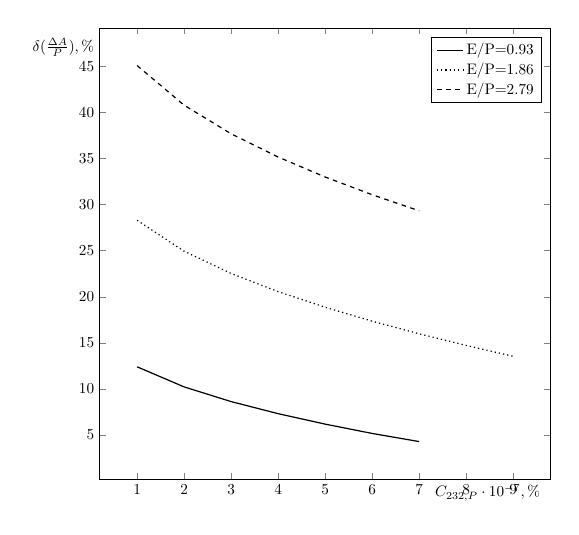
\begin{tikzpicture}[,
scale=0.55]
\begin{axis}[
  xlabel style = {{at={(axis description cs:.86,0)}}},
  ylabel = {$\delta(\frac{\Delta A}{P}), \%$},
  ylabel style = {{at={(axis description cs:-0.08,.925)},rotate=270,anchor=south}},
  xlabel = {$C_{232,P}\cdot10^{-7}, \%$},
  width=12cm, height=12cm
]

\addplot+[mark=none,
  solid, black, thick
] coordinates {
  (1.0, 12.395218440946906)
  (2.0, 10.219020529323354)
  (3.0000000000000004, 8.626929870001328)
  (4.0, 7.3185844692402915)
  (5.0, 6.185264012646069)
  (6.0, 5.173768588868835)
  (7.000000000000001, 4.29293979177781)
};
\addlegendentry{{}{E/P=0.93}}

\addplot+[mark=none,
  dotted, black, thick
] coordinates {
  (1.0, 28.282242175940937)
  (2.0, 24.929077234925025)
  (3.0000000000000004, 22.516662376271356)
  (4.0, 20.550634890717415)
  (5.0, 18.85615249546271)
  (6.0, 17.34800036201673)
  (7.000000000000001, 15.978805541243855)
  (8.0, 14.71681616393461)
  (9.000000000000002, 13.541592549068923)
};
\addlegendentry{{}{E/P=1.86}}

\addplot+[mark=none,
  dashed, black, thick
] coordinates {
  (1.0, 45.057945429681226)
  (2.0, 40.758242565718376)
  (3.0000000000000004, 37.66157309459905)
  (4.0, 35.14302713983917)
  (5.0, 32.97793340752656)
  (6.0, 31.056144200883885)
  (7.000000000000001, 29.31422868906391)
};
\addlegendentry{{}{E/P=2.79}}

\end{axis}
\end{tikzpicture}


      \caption{{Зависимость перерасхода работы разделения от ПДК $^{232}$U в НОУ-продукте с обогащением до уровня 4,4\% для различных $\frac{E}{P}${\label{sw44}}}}
    \end{minipage}%
    \begin{minipage}{.5\textwidth}
        \centering
        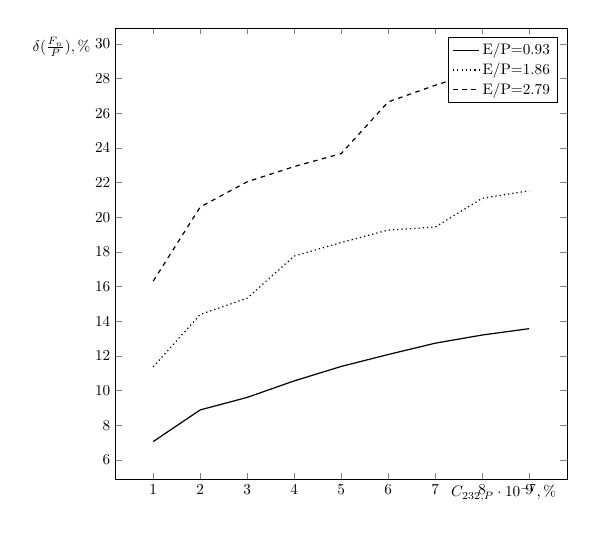
\begin{tikzpicture}[,
scale=0.55]
\begin{axis}[
  xlabel style = {{at={(axis description cs:.86,0)}}},
  ylabel = {$\delta(\frac{F_n}{P}), \%$},
  ylabel style = {{at={(axis description cs:-0.12,.925)},rotate=270,anchor=south}},
  xlabel = {$C_{232,P}\cdot10^{-7}, \%$},
  width=12cm, height=12cm
]

\addplot+[mark=none,
  solid, black, thick
] coordinates {
  (1.0, 7.057760090703368)
  (2.0, 8.883437157947327)
  (3.0000000000000004, 9.605444995054558)
  (4.0, 10.55710068193495)
  (5.0, 11.39016688359421)
  (6.0, 12.079179244566795)
  (7.000000000000001, 12.731349141503689)
  (8.0, 13.2030657848923)
  (9.000000000000002, 13.570378177156261)
};
\addlegendentry{{}{E/P=0.93}}

\addplot+[mark=none,
  dotted, black, thick
] coordinates {
  (1.0, 11.365686755446403)
  (2.0, 14.388303949542236)
  (3.0000000000000004, 15.32915753801609)
  (4.0, 17.755819239592196)
  (5.0, 18.538942955684167)
  (6.0, 19.25590180171489)
  (7.000000000000001, 19.428633887556103)
  (8.0, 21.089075670500623)
  (9.000000000000002, 21.52560986675717)
};
\addlegendentry{{}{E/P=1.86}}

\addplot+[mark=none,
  dashed, black, thick
] coordinates {
  (1.0, 16.31337535716355)
  (2.0, 20.58636758324206)
  (3.0000000000000004, 22.044054253914446)
  (4.0, 22.920132708437947)
  (5.0, 23.667999814578412)
  (6.0, 26.65031148325815)
  (7.000000000000001, 27.607494173667078)
  (8.0, 28.461707300289373)
  (9.000000000000002, 28.74364899102281)
};
\addlegendentry{{}{E/P=2.79}}

\end{axis}
\end{tikzpicture}

  \caption{{Зависимость расхода природного урана от ПДК $^{232}$U в НОУ-продукте с обогащением до уровня 4,4\% для различных $\frac{E}{P}${\label{F0R44}}}}
      \end{minipage}
\end{figure}

\begin{figure}
    \centering
    \begin{minipage}{.5\textwidth}
      \centering
      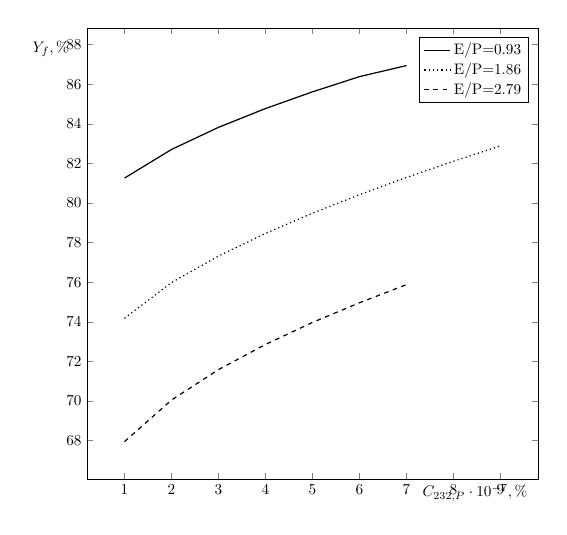
\begin{tikzpicture}[,
scale=0.55]
\begin{axis}[
  xlabel style = {{at={(axis description cs:.86,0)}}},
  ylabel = {$Y_{f}, \%$},
  ylabel style = {{at={(axis description cs:-0.08,.925)},rotate=270,anchor=south}},
  xlabel = {$C_{232,P}\cdot10^{-7}, \%$},
  width=12cm, height=12cm
]

\addplot+[mark=none,
  solid, black, thick
] coordinates {
  (1.0, 81.2599146274243)
  (2.0, 82.70510635581616)
  (3.0000000000000004, 83.82183689954859)
  (4.0, 84.77127401369083)
  (5.0, 85.61487919146296)
  (6.0, 86.38356067088392)
  (7.000000000000001, 86.94074198596759)
};
\addlegendentry{{}{E/P=0.93}}

\addplot+[mark=none,
  dotted, black, thick
] coordinates {
  (1.0, 74.17655829999579)
  (2.0, 75.98498213201852)
  (3.0000000000000004, 77.32265969408223)
  (4.0, 78.46540402752339)
  (5.0, 79.48580928842689)
  (6.0, 80.42063662698051)
  (7.000000000000001, 81.29053109508794)
  (8.0, 82.1100269832236)
  (9.000000000000002, 82.88835691546974)
};
\addlegendentry{{}{E/P=1.86}}

\addplot+[mark=none,
  dashed, black, thick
] coordinates {
  (1.0, 67.95360281561639)
  (2.0, 70.05234164130057)
  (3.0000000000000004, 71.58870177419513)
  (4.0, 72.85958391192455)
  (5.0, 73.97031718490105)
  (6.0, 74.96387446964957)
  (7.000000000000001, 75.87957963032518)
};
\addlegendentry{{}{E/P=2.79}}

\end{axis}
\end{tikzpicture}


      \caption{{Зависимость степени извлечения $^{235}$U из регенерата от ПДК $^{232}$U в НОУ-продукте с обогащением до уровня 4,4\% для различных $\frac{E}{P}${\label{exR44}}}}
    \end{minipage}%
    \begin{minipage}{.5\textwidth}
        \centering
        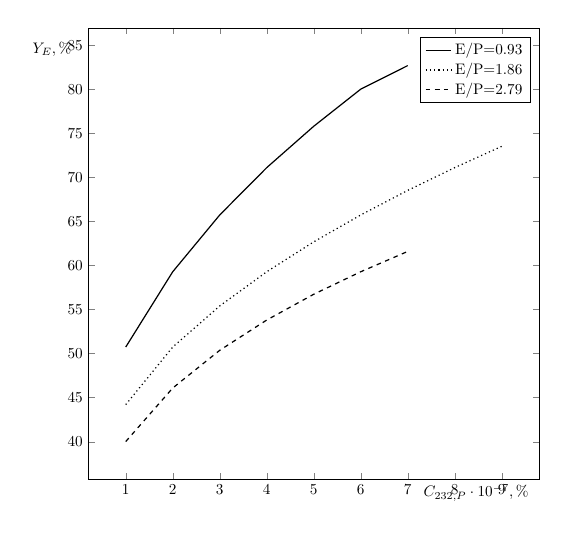
\begin{tikzpicture}[,
scale=0.55]
\begin{axis}[
  xlabel style = {{at={(axis description cs:.86,0)}}},
  ylabel = {$Y_{E}, \%$},
  ylabel style = {{at={(axis description cs:-0.08,.925)},rotate=270,anchor=south}},
  xlabel = {$C_{232,P}\cdot10^{-7}, \%$},
  width=12cm, height=12cm
]

\addplot+[mark=none,
  solid, black, thick
] coordinates {
  (1.0, 50.745320366220234)
  (2.0, 59.30149726322195)
  (3.0000000000000004, 65.7519664106782)
  (4.0, 71.12954522207235)
  (5.0, 75.82763880377072)
  (6.0, 80.04430359281832)
  (7.000000000000001, 82.72459665893969)
};
\addlegendentry{{}{E/P=0.93}}

\addplot+[mark=none,
  dotted, black, thick
] coordinates {
  (1.0, 44.20353110984807)
  (2.0, 50.745320366220234)
  (3.0000000000000004, 55.41327633341921)
  (4.0, 59.30149726322195)
  (5.0, 62.69903149138577)
  (6.0, 65.75196641067834)
  (7.000000000000001, 68.5430309981216)
  (8.0, 71.12954522207235)
  (9.000000000000002, 73.54852477832327)
};
\addlegendentry{{}{E/P=1.86}}

\addplot+[mark=none,
  dashed, black, thick
] coordinates {
  (1.0, 40.009414250517715)
  (2.0, 46.09394772079198)
  (3.0000000000000004, 50.37816062607195)
  (4.0, 53.81590263606467)
  (5.0, 56.74369030977263)
  (6.0, 59.30149726322191)
  (7.000000000000001, 61.61037730716592)
};
\addlegendentry{{}{E/P=2.79}}

\end{axis}
\end{tikzpicture}


        \caption{{Зависимость степени извлечения $^{235}$U из регенерата от ПДК $^{232}$U в НОУ-продукте с обогащением до уровня 4,4\% для различных $\frac{E}{P}${\label{exR44}}}}
      \end{minipage}
\end{figure}

\begin{figure}
    \centering
    \begin{minipage}{.5\textwidth}
      \centering
      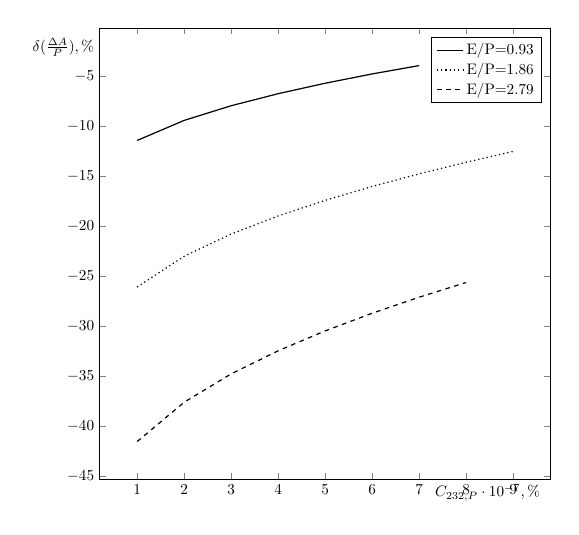
\begin{tikzpicture}[,
scale=0.55]
\begin{axis}[
  xlabel style = {{at={(axis description cs:.86,0)}}},
  ylabel = {$\delta(\frac{\Delta A}{P}), \%$},
  ylabel style = {{at={(axis description cs:-0.08,.925)},rotate=270,anchor=south}},
  xlabel = {$C_{232,P}\cdot10^{-7}, \%$},
  width=12cm, height=12cm
]

\addplot+[mark=none,
  solid, black, thick
] coordinates {
  (1.0, -11.442050325962452)
  (2.0, -9.438723200431037)
  (3.0000000000000004, -7.9728246964313)
  (4.0, -6.768022196914314)
  (5.0, -5.7242794711367315)
  (6.0, -4.7922989130984135)
  (7.000000000000001, -3.956523255555432)
};
\addlegendentry{{}{E/P=0.93}}

\addplot+[mark=none,
  dotted, black, thick
] coordinates {
  (1.0, -26.09957395082424)
  (2.0, -23.022672963318332)
  (3.0000000000000004, -20.802863046158134)
  (4.0, -18.993519736891432)
  (5.0, -17.43387788617293)
  (6.0, -16.045572170953353)
  (7.000000000000001, -14.785062105867015)
  (8.0, -13.623128278493162)
  (9.000000000000002, -12.541001761914492)
};
\addlegendentry{{}{E/P=1.86}}

\addplot+[mark=none,
  dashed, black, thick
] coordinates {
  (1.0, -41.554133458995025)
  (2.0, -37.62214258113987)
  (3.0000000000000004, -34.78539667116384)
  (4.0, -32.475395453374304)
  (5.0, -30.487594682338603)
  (6.0, -28.721514147914533)
  (7.000000000000001, -27.11944341607787)
  (8.0, -25.644440494125277)
};
\addlegendentry{{}{E/P=2.79}}

\end{axis}
\end{tikzpicture}


\caption{{Зависимость перерасхода работы разделения от ПДК $^{232}$U в НОУ-продукте с обогащением до уровня 4,7\% для различных $\frac{E}{P}${\label{sw47}}}}
    \end{minipage}%
    \begin{minipage}{.5\textwidth}
        \centering
        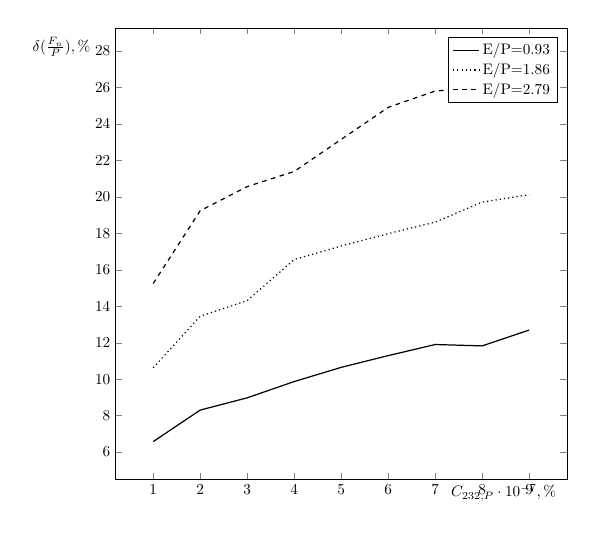
\begin{tikzpicture}[,
scale=0.55]
\begin{axis}[
  xlabel style = {{at={(axis description cs:.86,0)}}},
  ylabel = {$\delta(\frac{F_n}{P}), \%$},
  ylabel style = {{at={(axis description cs:-0.12,.925)},rotate=270,anchor=south}},
  xlabel = {$C_{232,P}\cdot10^{-7}, \%$},
  width=12cm, height=12cm
]

\addplot+[mark=none,
  solid, black, thick
] coordinates {
  (1.0, 6.575777960449747)
  (2.0, 8.304082560693814)
  (3.0000000000000004, 8.976090710675233)
  (4.0, 9.868594115237716)
  (5.0, 10.647329915250959)
  (6.0, 11.291406719065089)
  (7.000000000000001, 11.901043804010158)
  (8.0, 11.825222422159886)
  (9.000000000000002, 12.695878057693244)
};
\addlegendentry{{}{E/P=0.93}}

\addplot+[mark=none,
  dotted, black, thick
] coordinates {
  (1.0, 10.624446333883753)
  (2.0, 13.449936300634558)
  (3.0000000000000004, 14.311239719353042)
  (4.0, 16.560710478871865)
  (5.0, 17.306489772128366)
  (6.0, 17.983340260297208)
  (7.000000000000001, 18.616420256437195)
  (8.0, 19.71370096673143)
  (9.000000000000002, 20.121765534932436)
};
\addlegendentry{{}{E/P=1.86}}

\addplot+[mark=none,
  dashed, black, thick
] coordinates {
  (1.0, 15.24945962762343)
  (2.0, 19.243778391551892)
  (3.0000000000000004, 20.565609869945966)
  (4.0, 21.396074588142078)
  (6.0, 24.912247692066092)
  (7.000000000000001, 25.8070054249773)
  (8.0, 26.023713660172486)
  (9.000000000000002, 27.20442149271206)
};
\addlegendentry{{}{E/P=2.79}}

\end{axis}
\end{tikzpicture}

    \caption{{Зависимость расхода природного урана от ПДК $^{232}$U в НОУ-продукте с обогащением до уровня 4,7\% для различных $\frac{E}{P}${\label{F0R47}}}}
    \end{minipage}
\end{figure}

\begin{figure}
    \centering
    \begin{minipage}{.5\textwidth}
      \centering
      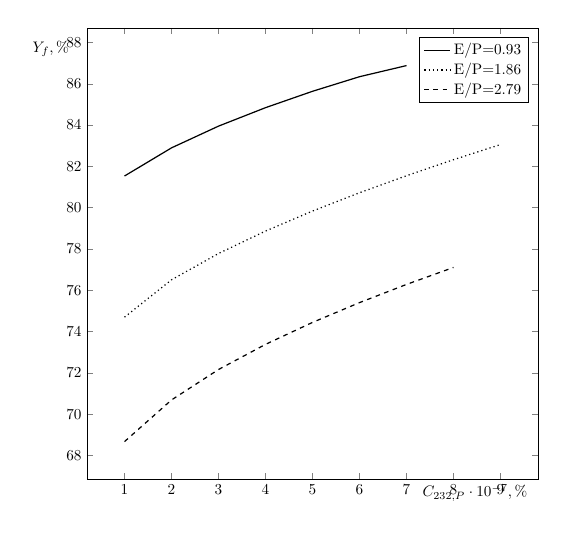
\begin{tikzpicture}[,
scale=0.55]
\begin{axis}[
  xlabel style = {{at={(axis description cs:.86,0)}}},
  ylabel = {$Y_{f}, \%$},
  ylabel style = {{at={(axis description cs:-0.08,.925)},rotate=270,anchor=south}},
  xlabel = {$C_{232,P}\cdot10^{-7}, \%$},
  width=12cm, height=12cm
]

\addplot+[mark=none,
  solid, black, thick
] coordinates {
  (1.0, 81.53156037359754)
  (2.0, 82.89545086273719)
  (3.0000000000000004, 83.9478345607235)
  (4.0, 84.84152401044177)
  (5.0, 85.63479347902604)
  (6.0, 86.3412156692256)
  (7.000000000000001, 86.88027992336104)
};
\addlegendentry{{}{E/P=0.93}}

\addplot+[mark=none,
  dotted, black, thick
] coordinates {
  (1.0, 74.69415676339759)
  (2.0, 76.50476826786495)
  (3.0000000000000004, 77.77849512744808)
  (4.0, 78.86515635925242)
  (5.0, 79.83436020530084)
  (6.0, 80.72135365193532)
  (7.000000000000001, 81.54594313296484)
  (8.0, 82.32205886834831)
  (9.000000000000002, 83.05589060957709)
};
\addlegendentry{{}{E/P=1.86}}

\addplot+[mark=none,
  dashed, black, thick
] coordinates {
  (1.0, 68.6697629941284)
  (2.0, 70.68575248489067)
  (3.0000000000000004, 72.15973261088106)
  (4.0, 73.37774759491083)
  (5.0, 74.44135268684659)
  (6.0, 75.39965734146578)
  (7.000000000000001, 76.28121651908731)
  (8.0, 77.10358771087932)
};
\addlegendentry{{}{E/P=2.79}}

\end{axis}
\end{tikzpicture}


      \caption{{Зависимость степени извлечения $^{235}$U от ПДК $^{232}$U в НОУ-продукте с обогащением до уровня 4,7\% для различных $\frac{E}{P}${\label{ex47}}}}
    \end{minipage}%
    \begin{minipage}{.5\textwidth}
        \centering
        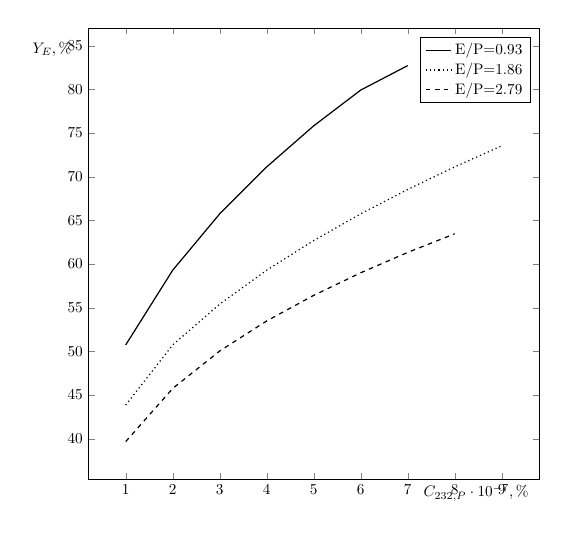
\begin{tikzpicture}[,
scale=0.55]
\begin{axis}[
  xlabel style = {{at={(axis description cs:.86,0)}}},
  ylabel = {$Y_{E}, \%$},
  ylabel style = {{at={(axis description cs:-0.08,.925)},rotate=270,anchor=south}},
  xlabel = {$C_{232,P}\cdot10^{-7}, \%$},
  width=12cm, height=12cm
]

\addplot+[mark=none,
  solid, black, thick
] coordinates {
  (1.0, 50.74532036622023)
  (2.0, 59.30149726322195)
  (3.0000000000000004, 65.75196641067834)
  (4.0, 71.12954522207235)
  (5.0, 75.82763880377072)
  (6.0, 79.9222355420343)
  (7.000000000000001, 82.72736369212772)
};
\addlegendentry{{}{E/P=0.93}}

\addplot+[mark=none,
  dotted, black, thick
] coordinates {
  (1.0, 43.8508093556669)
  (2.0, 50.745320366220234)
  (3.0000000000000004, 55.41327633341921)
  (4.0, 59.30149726322195)
  (5.0, 62.699031491385725)
  (6.0, 65.75196641067818)
  (7.000000000000001, 68.5430309981216)
  (8.0, 71.12954522207235)
  (9.000000000000002, 73.53797277442622)
};
\addlegendentry{{}{E/P=1.86}}

\addplot+[mark=none,
  dashed, black, thick
] coordinates {
  (1.0, 39.675583995839325)
  (2.0, 45.761133085161255)
  (3.0000000000000004, 50.047914553011395)
  (4.0, 53.488618646439654)
  (5.0, 56.419645475250455)
  (6.0, 59.003049808125226)
  (7.000000000000001, 61.33254693680554)
  (8.0, 63.465686451699256)
};
\addlegendentry{{}{E/P=2.79}}

\end{axis}
\end{tikzpicture}


        \caption{{Зависимость степени извлечения $^{235}$U из регенерата от ПДК $^{232}$U в НОУ-продукте с обогащением до уровня 4,7\% для различных $\frac{E}{P}${\label{exR47}}}}
    \end{minipage}
\end{figure}

\begin{figure}
    \centering
    \begin{minipage}{.5\textwidth}
      \centering
      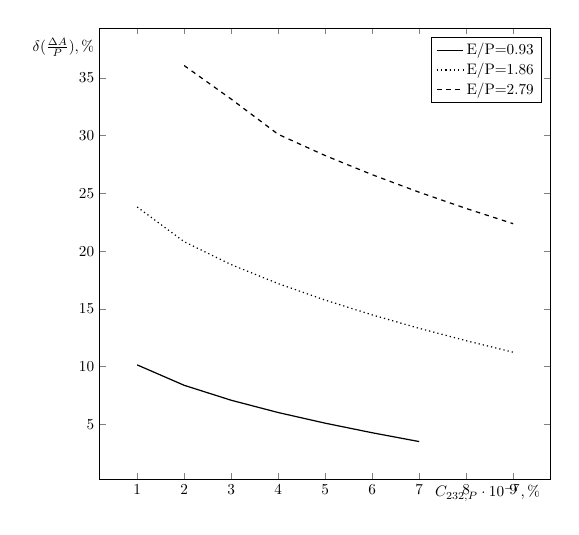
\begin{tikzpicture}[,
scale=0.55]
\begin{axis}[
  xlabel style = {{at={(axis description cs:.86,0)}}},
  ylabel = {$\delta(\frac{\Delta A}{P}), \%$},
  ylabel style = {{at={(axis description cs:-0.08,.925)},rotate=270,anchor=south}},
  xlabel = {$C_{232,P}\cdot10^{-7}, \%$},
  width=12cm, height=12cm
]

\addplot+[mark=none,
  solid, black, thick
] coordinates {
  (1.0, 10.149838341711135)
  (2.0, 8.382155711990722)
  (3.0000000000000004, 7.088371632908093)
  (4.0, 6.0248508842357245)
  (5.0, 5.102882323296978)
  (6.0, 4.273113201042603)
  (7.000000000000001, 3.509602428442813)
};
\addlegendentry{{}{E/P=0.93}}

\addplot+[mark=none,
  dotted, black, thick
] coordinates {
  (1.0, 23.823133024898677)
  (2.0, 20.815838403670245)
  (3.0000000000000004, 18.832982700086603)
  (4.0, 17.18881625250314)
  (5.0, 15.758547005316414)
  (6.0, 14.479894930684239)
  (7.000000000000001, 13.316185752259024)
  (8.0, 12.243723663525396)
  (9.000000000000002, 11.246222146183511)
};
\addlegendentry{{}{E/P=1.86}}

\addplot+[mark=none,
  dashed, black, thick
] coordinates {
  (2.0, 36.066525267783106)
  (3.0000000000000004, 33.16682579758896)
  (4.0, 30.115313378877072)
  (5.0, 28.275805724474395)
  (6.0, 26.618567158713446)
  (7.000000000000001, 25.10030828410702)
  (8.0, 23.692935156588334)
  (9.000000000000002, 22.376908192213214)
};
\addlegendentry{{}{E/P=2.79}}

\end{axis}
\end{tikzpicture}


      \caption{{Зависимость перерасхода работы разделения от ПДК $^{232}$U в НОУ-продукте с обогащением до уровня 5,2\% для различных $\frac{E}{P}${\label{sw52}}}}
    \end{minipage}%
    \begin{minipage}{.5\textwidth}
      \centering
      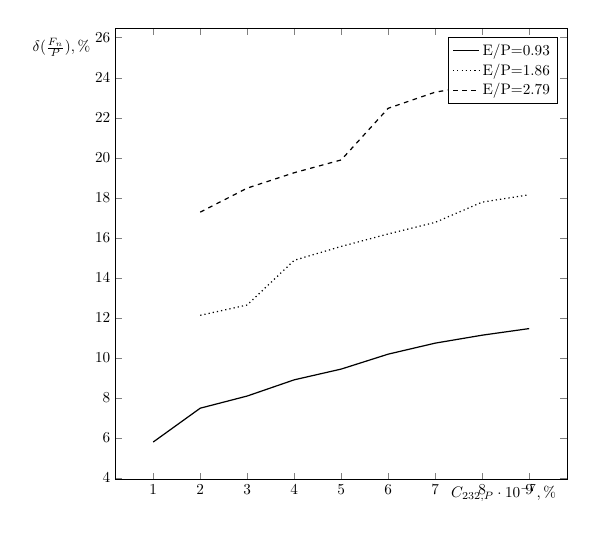
\begin{tikzpicture}[,
scale=0.55]
\begin{axis}[
  xlabel style = {{at={(axis description cs:.86,0)}}},
  ylabel = {$\delta(\frac{F_n}{P}), \%$},
  ylabel style = {{at={(axis description cs:-0.12,.925)},rotate=270,anchor=south}},
  xlabel = {$C_{232,P}\cdot10^{-7}, \%$},
  width=12cm, height=12cm
]

\addplot+[mark=none,
  solid, black, thick
] coordinates {
  (1.0, 5.793046394428947)
  (2.0, 7.4830576011553855)
  (3.0000000000000004, 8.091358069070598)
  (4.0, 8.901084905310231)
  (5.0, 9.438059464830372)
  (6.0, 10.18430556091351)
  (7.000000000000001, 10.734274883113482)
  (8.0, 11.131996659369692)
  (9.000000000000002, 11.461858128710666)
};
\addlegendentry{{}{E/P=0.93}}

\addplot+[mark=none,
  dotted, black, thick
] coordinates {
  (2.0, 12.123287852615794)
  (3.0000000000000004, 12.641245614364582)
  (4.0, 14.874069679925771)
  (5.0, 15.566658207311013)
  (6.0, 16.191082381194388)
  (7.000000000000001, 16.769702434887257)
  (8.0, 17.780984910214105)
  (9.000000000000002, 18.14904312365678)
};
\addlegendentry{{}{E/P=1.86}}

\addplot+[mark=none,
  dashed, black, thick
] coordinates {
  (2.0, 17.28090551539224)
  (3.0000000000000004, 18.480641817808085)
  (4.0, 19.250290190147645)
  (5.0, 19.889420973493365)
  (6.0, 22.4698704842767)
  (7.000000000000001, 23.276906871527515)
  (8.0, 23.66795997375587)
  (9.000000000000002, 24.581976879770806)
};
\addlegendentry{{}{E/P=2.79}}

\end{axis}
\end{tikzpicture}


    \caption{{Зависимость расхода природного урана от ПДК $^{232}$U в НОУ-продукте с обогащением до уровня 5,2\% для различных $\frac{E}{P}${\label{F0R52}}}}
    \end{minipage}
\end{figure}

\begin{figure}
    \centering
    \begin{minipage}{.5\textwidth}
      \centering
      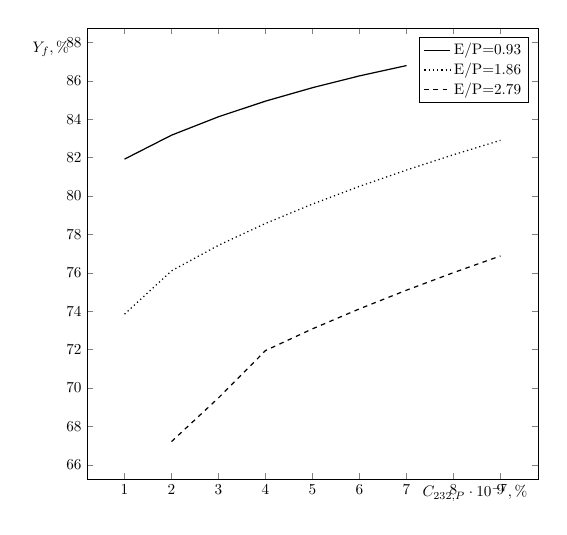
\begin{tikzpicture}[,
scale=0.55]
\begin{axis}[
  xlabel style = {{at={(axis description cs:.86,0)}}},
  ylabel = {$Y_{f}, \%$},
  ylabel style = {{at={(axis description cs:-0.08,.925)},rotate=270,anchor=south}},
  xlabel = {$C_{232,P}\cdot10^{-7}, \%$},
  width=12cm, height=12cm
]

\addplot+[mark=none,
  solid, black, thick
] coordinates {
  (1.0, 81.92047282281692)
  (2.0, 83.16742538966415)
  (3.0000000000000004, 84.12759194071681)
  (4.0, 84.94161765082885)
  (5.0, 85.64166453585005)
  (6.0, 86.25729994352187)
  (7.000000000000001, 86.79329916754914)
};
\addlegendentry{{}{E/P=0.93}}

\addplot+[mark=none,
  dotted, black, thick
] coordinates {
  (1.0, 73.84598056878988)
  (2.0, 76.10056358211024)
  (3.0000000000000004, 77.43294968555689)
  (4.0, 78.56987165120975)
  (5.0, 79.5809470624556)
  (6.0, 80.50160145898167)
  (7.000000000000001, 81.35303037639089)
  (8.0, 82.14905252951476)
  (9.000000000000002, 82.89921358322908)
};
\addlegendentry{{}{E/P=1.86}}

\addplot+[mark=none,
  dashed, black, thick
] coordinates {
  (2.0, 67.20594201450372)
  (3.0000000000000004, 69.48318645671289)
  (4.0, 71.94804280408532)
  (5.0, 73.08027680473819)
  (6.0, 74.12135493795347)
  (7.000000000000001, 75.09259182720001)
  (8.0, 76.00791338569806)
  (9.000000000000002, 76.87705901175764)
};
\addlegendentry{{}{E/P=2.79}}

\end{axis}
\end{tikzpicture}


      \caption{{Зависимость степени извлечения $^{235}$U из регенерата от ПДК $^{232}$U в НОУ-продукте с обогащением до уровня 5,2\% для различных $\frac{E}{P}${\label{exR52}}}}
    \end{minipage}%
    \begin{minipage}{.5\textwidth}
      \centering
      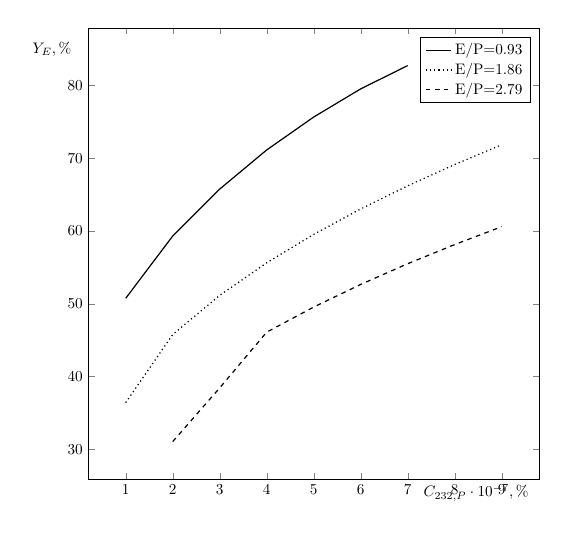
\begin{tikzpicture}[,
scale=0.55]
\begin{axis}[
  xlabel style = {{at={(axis description cs:.86,0)}}},
  ylabel = {$Y_{E}, \%$},
  ylabel style = {{at={(axis description cs:-0.08,.925)},rotate=270,anchor=south}},
  xlabel = {$C_{232,P}\cdot10^{-7}, \%$},
  width=12cm, height=12cm
]

\addplot+[mark=none,
  solid, black, thick
] coordinates {
  (1.0, 50.745320366220206)
  (2.0, 59.30149726322206)
  (3.0000000000000004, 65.75196641067834)
  (4.0, 71.1295452220723)
  (5.0, 75.6532981285366)
  (6.0, 79.52272196391077)
  (7.000000000000001, 82.72253492281729)
};
\addlegendentry{{}{E/P=0.93}}

\addplot+[mark=none,
  dotted, black, thick
] coordinates {
  (1.0, 36.4111106586823)
  (2.0, 45.76462199063639)
  (3.0000000000000004, 51.14102895339182)
  (4.0, 55.622818080555916)
  (5.0, 59.52901295979165)
  (6.0, 63.02235936849755)
  (7.000000000000001, 66.20030038850088)
  (8.0, 69.12649182519807)
  (9.000000000000002, 71.84506168392848)
};
\addlegendentry{{}{E/P=1.86}}

\addplot+[mark=none,
  dashed, black, thick
] coordinates {
  (2.0, 31.052928837106435)
  (3.0000000000000004, 38.434804849560365)
  (4.0, 46.09143609388377)
  (5.0, 49.541981912692776)
  (6.0, 52.64930445174624)
  (7.000000000000001, 55.493065127672466)
  (8.0, 58.12552740420125)
  (9.000000000000002, 60.58336009265791)
};
\addlegendentry{{}{E/P=2.79}}

\end{axis}
\end{tikzpicture}


      \caption{{Зависимость степени извлечения $^{235}$U из регенерата от ПДК $^{232}$U в НОУ-продукте с обогащением до уровня 5,2\% для различных $\frac{E}{P}${\label{exR52}}}}
    \end{minipage}
\end{figure}

\begin{figure}
    \centering
    \begin{minipage}{.5\textwidth}
      \centering
      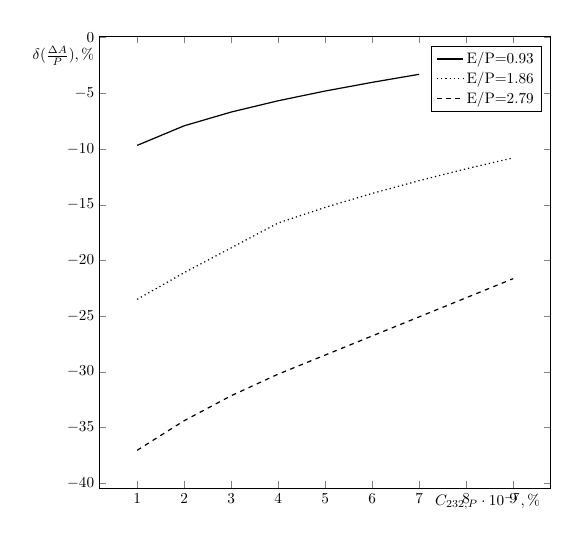
\begin{tikzpicture}[,
scale=0.55]
\begin{axis}[
  xlabel style = {{at={(axis description cs:.86,0)}}},
  ylabel = {$\delta(\frac{\Delta A}{P}), \%$},
  ylabel style = {{at={(axis description cs:-0.08,.925)},rotate=270,anchor=south}},
  xlabel = {$C_{232,P}\cdot10^{-7}, \%$},
  width=12cm, height=12cm
]

\addplot+[mark=none,
  solid, black, thick
] coordinates {
  (1.0, -9.674911908891808)
  (2.0, -7.916580534549614)
  (3.0000000000000004, -6.681867721811178)
  (4.0, -5.6678082447103755)
  (5.0, -4.794275755390127)
  (6.0, -4.014408958772108)
  (7.000000000000001, -3.2916785299194777)
};
\addlegendentry{{}{E/P=0.93}}

\addplot+[mark=none,
  dotted, black, thick
] coordinates {
  (1.0, -23.50106092571201)
  (2.0, -21.106953058591188)
  (3.0000000000000004, -18.88217189205597)
  (4.0, -16.643364366696886)
  (5.0, -15.246115172124236)
  (6.0, -13.990185059339408)
  (7.000000000000001, -12.842927411164878)
  (8.0, -11.782798941270507)
  (9.000000000000002, -10.794662240262344)
};
\addlegendentry{{}{E/P=1.86}}

\addplot+[mark=none,
  dashed, black, thick
] coordinates {
  (1.0, -37.05851569736411)
  (2.0, -34.40029262029973)
  (3.0000000000000004, -32.15953244222282)
  (4.0, -30.21936688019669)
  (9.000000000000002, -21.645943926803636)
};
\addlegendentry{{}{E/P=2.79}}

\end{axis}
\end{tikzpicture}


\caption{{Зависимость перерасхода работы разделения от ПДК $^{232}$U в НОУ-продукте с обогащением до уровня 5,5\% для различных $\frac{E}{P}${\label{sw55}}}}
    \end{minipage}%
    \begin{minipage}{.5\textwidth}
      \centering
      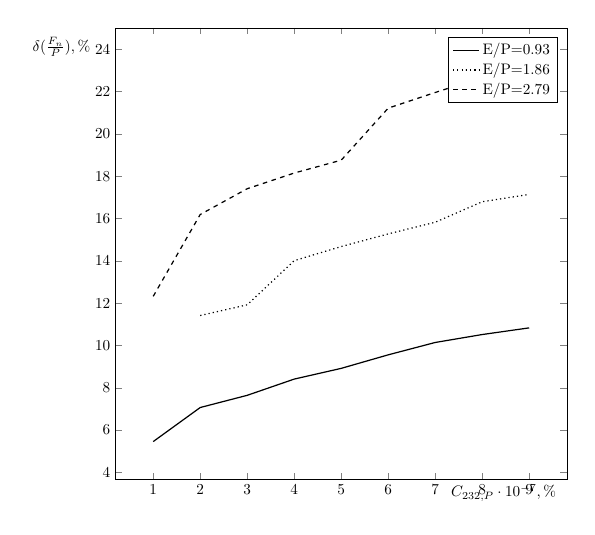
\begin{tikzpicture}[,
scale=0.55]
\begin{axis}[
  xlabel style = {{at={(axis description cs:.86,0)}}},
  ylabel = {$\delta(\frac{F_n}{P}), \%$},
  ylabel style = {{at={(axis description cs:-0.12,.925)},rotate=270,anchor=south}},
  xlabel = {$C_{232,P}\cdot10^{-7}, \%$},
  width=12cm, height=12cm
]

\addplot+[mark=none,
  solid, black, thick
] coordinates {
  (1.0, 5.4518852373011235)
  (2.0, 7.062106446811822)
  (3.0000000000000004, 7.6389396471428395)
  (4.0, 8.406580615825042)
  (5.0, 8.91372326597052)
  (6.0, 9.553487958028839)
  (7.000000000000001, 10.137926733330982)
  (8.0, 10.513552818081562)
  (9.000000000000002, 10.828975022060794)
};
\addlegendentry{{}{E/P=0.93}}

\addplot+[mark=none,
  dotted, black, thick
] coordinates {
  (2.0, 11.4125628071713)
  (3.0000000000000004, 11.919207344081862)
  (4.0, 14.00682887106841)
  (5.0, 14.67424564867117)
  (6.0, 15.272445794132029)
  (7.000000000000001, 15.824088637039257)
  (8.0, 16.793152631424558)
  (9.000000000000002, 17.14076317272052)
};
\addlegendentry{{}{E/P=1.86}}

\addplot+[mark=none,
  dashed, black, thick
] coordinates {
  (1.0, 12.320069331258377)
  (2.0, 16.18989448953321)
  (3.0000000000000004, 17.409881282949357)
  (4.0, 18.15088017430695)
  (5.0, 18.758892682933727)
  (6.0, 21.219879210414405)
  (7.000000000000001, 21.960274322729067)
  (8.0, 22.671364365359803)
  (9.000000000000002, 23.232704136321768)
};
\addlegendentry{{}{E/P=2.79}}

\end{axis}
\end{tikzpicture}


    \caption{{Зависимость расхода природного урана от ПДК $^{232}$U в НОУ-продукте с обогащением до уровня 5,5\% для различных $\frac{E}{P}${\label{F0R55}}}}
\end{minipage}
\end{figure}

\begin{figure}
    \centering
    \begin{minipage}{.5\textwidth}
      \centering
      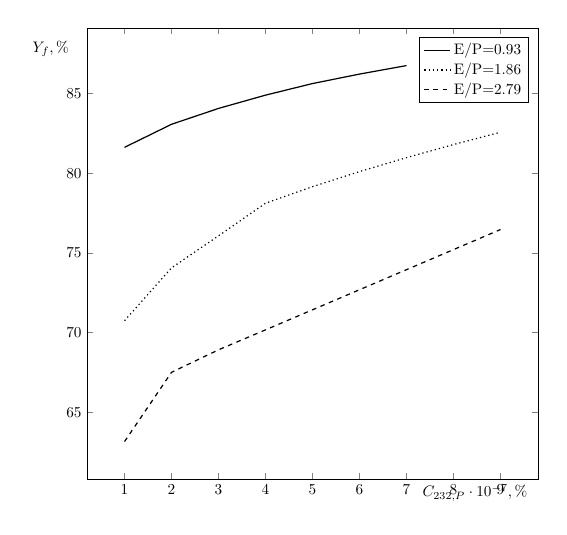
\begin{tikzpicture}[,
scale=0.55]
\begin{axis}[
  xlabel style = {{at={(axis description cs:.86,0)}}},
  ylabel = {$Y_{f}, \%$},
  ylabel style = {{at={(axis description cs:-0.08,.925)},rotate=270,anchor=south}},
  xlabel = {$C_{232,P}\cdot10^{-7}, \%$},
  width=12cm, height=12cm
]

\addplot+[mark=none,
  solid, black, thick
] coordinates {
  (1.0, 81.61991908264207)
  (2.0, 83.06585782673034)
  (3.0000000000000004, 84.06121871723813)
  (4.0, 84.89394884244733)
  (5.0, 85.62112811640561)
  (6.0, 86.21532750169558)
  (7.000000000000001, 86.74881397482362)
};
\addlegendentry{{}{E/P=0.93}}

\addplot+[mark=none,
  dotted, black, thick
] coordinates {
  (1.0, 70.74596601492043)
  (2.0, 74.06158601844446)
  (3.0000000000000004, 76.06862560997918)
  (4.0, 78.11684252280332)
  (5.0, 79.15281009487043)
  (6.0, 80.09858956685858)
  (7.000000000000001, 80.97460907120315)
  (8.0, 81.7944538096466)
  (9.000000000000002, 82.56771088986454)
};
\addlegendentry{{}{E/P=1.86}}

\addplot+[mark=none,
  dashed, black, thick
] coordinates {
  (1.0, 63.16381724872306)
  (2.0, 67.50888937364991)
  (3.0000000000000004, 68.91979697654483)
  (4.0, 70.1710975477616)
  (9.000000000000002, 76.46473227843333)
};
\addlegendentry{{}{E/P=2.79}}

\end{axis}
\end{tikzpicture}


      \caption{{Зависимость степени извлечения $^{235}$U от ПДК $^{232}$U в НОУ-продукте с обогащением до уровня 5,5\% для различных $\frac{E}{P}${\label{ex55}}}}
    \end{minipage}%
    \begin{minipage}{.5\textwidth}
      \centering
      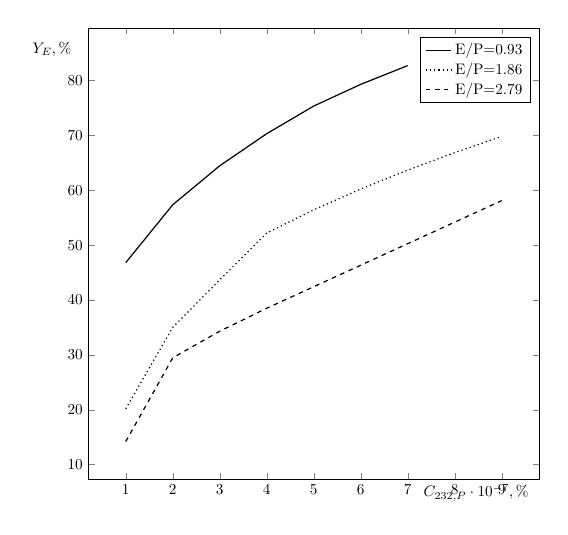
\begin{tikzpicture}[,
scale=0.55]
\begin{axis}[
  xlabel style = {{at={(axis description cs:.86,0)}}},
  ylabel = {$Y_{E}, \%$},
  ylabel style = {{at={(axis description cs:-0.08,.925)},rotate=270,anchor=south}},
  xlabel = {$C_{232,P}\cdot10^{-7}, \%$},
  width=12cm, height=12cm
]

\addplot+[mark=none,
  solid, black, thick
] coordinates {
  (1.0, 46.800208774629716)
  (2.0, 57.35033934688334)
  (3.0000000000000004, 64.45948860219971)
  (4.0, 70.30908697025141)
  (5.0, 75.34542620989228)
  (6.0, 79.29919036071507)
  (7.000000000000001, 82.723141968642)
};
\addlegendentry{{}{E/P=0.93}}

\addplot+[mark=none,
  dotted, black, thick
] coordinates {
  (1.0, 20.160926232575846)
  (2.0, 35.007223506049215)
  (3.0000000000000004, 43.66597559028209)
  (4.0, 52.200316349986885)
  (5.0, 56.42853055286887)
  (6.0, 60.21940831661349)
  (7.000000000000001, 63.672842081572945)
  (8.0, 66.85533055225017)
  (9.000000000000002, 69.81385047110462)
};
\addlegendentry{{}{E/P=1.86}}

\addplot+[mark=none,
  dashed, black, thick
] coordinates {
  (1.0, 14.192755424067755)
  (2.0, 29.457231870306288)
  (3.0000000000000004, 34.301390009573225)
  (4.0, 38.492060382311266)
  (9.000000000000002, 58.11121612024639)
};
\addlegendentry{{}{E/P=2.79}}

\end{axis}
\end{tikzpicture}


      \caption{{Зависимость степени извлечения $^{235}$U из регенерата от ПДК $^{232}$U в НОУ-продукте с обогащением до уровня 5,5\% для различных $\frac{E}{P}${\label{exR55}}}}
\end{minipage}
\end{figure}



% \chapter*{Приложение Г}       % Заголовок
% \addcontentsline{toc}{chapter}{Приложение Г. Схема двойного каскада с НОУ-разбавителем с возвратом потока $P_2$ в цикл. Дополнительные результаты}
% \noindent

% % \counterwithin{figure}{chapter}
% % \counterwithin{table}{chapter}
% \renewcommand{\thefigure}{Г\arabic{figure}}
% \setcounter{figure}{0}
% \renewcommand{\thetable}{Г\arabic{table}}
% \setcounter{table}{0}

% \textbf{Схема двойного каскада с НОУ-разбавителем с возвратом потока $P_2$ в цикл. Дополнительные результаты для состава 1}

% При варьировании опорного $k$-го компонента.

% \begin{figure}[ht]
%     \centering
%     \begin{minipage}{.5\textwidth}
%       \centering
%       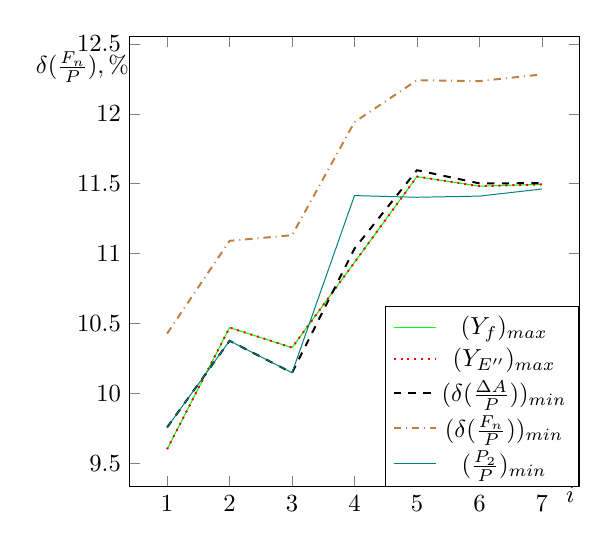
\begin{tikzpicture}[,
scale=0.89]
\begin{axis}[
  xlabel style = {{at={(axis description cs:.98,0.02)}}},
  ylabel = {$\delta(\frac{F_n}{P}), \%$},
  ylabel style = {{at={(axis description cs:-0.105,.88)},rotate=270,anchor=south}},
  xlabel = {$i$},
  width=8cm, height=8cm, xtick={1,2,3,4,5,6,7}, legend style={at={(1,0)},anchor=south east}
]

\addplot+[mark=none,
  solid, green, thin
] coordinates {
  (1.0, 9.60224940765123)
  (2.0, 10.471964607421514)
  (3.0, 10.328677265019726)
  (4.0, 10.937722799772365)
  (5.0, 11.551073258460454)
  (6.0, 11.482634526238378)
  (7.0, 11.495414262020132)
};
\addlegendentry{{}{$(Y_f)_\text{max}$}}

\addplot+[mark=none,
  dotted, red, thick
] coordinates {
  (1.0, 9.60224940765123)
  (2.0, 10.471964607421514)
  (3.0, 10.328677265019726)
  (4.0, 10.937722799772365)
  (5.0, 11.551073258460454)
  (6.0, 11.482634526238378)
  (7.0, 11.495414262020132)
};
\addlegendentry{{}{$(Y_{E''})_\text{max}$}}

\addplot+[mark=none,
  dashed, black, thick
] coordinates {
  (1.0, 9.758344663807906)
  (2.0, 10.377586059230682)
  (3.0, 10.148945832377942)
  (4.0, 11.036603656094378)
  (5.0, 11.596700175896046)
  (6.0, 11.502422364899322)
  (7.0, 11.5042389394856)
};
\addlegendentry{{}{$(\delta(\frac{\Delta A}{P}))_\text{min}$}}

\addplot+[mark=none,
  dashdotted, brown, thick
] coordinates {
  (1.0, 10.428757919569875)
  (2.0, 11.091940883100326)
  (3.0, 11.132231272182302)
  (4.0, 11.940825541138867)
  (5.0, 12.240045586112991)
  (6.0, 12.233596137265634)
  (7.0, 12.281186997924387)
};
\addlegendentry{{}{$(\delta(\frac{F_n}{P}))_\text{min}$}}

\addplot+[mark=none,
  solid, teal, thin
] coordinates {
  (1.0, 9.758344663807906)
  (2.0, 10.377586059230682)
  (3.0, 10.148945832377942)
  (4.0, 11.415331124937522)
  (5.0, 11.403205816515582)
  (6.0, 11.411528711119201)
  (7.0, 11.462271406331004)
};
\addlegendentry{{}{$(\frac{P_2}{P})_\text{min}$}}

\end{axis}
\end{tikzpicture}


%       \caption{{Зависимость экономии природного урана в двойном каскаде с замыканием от номера перегрузки для различных критериев оптимальности. ($C_{235,{P}}=4,95\%$){\label{3}}}}
%     \end{minipage}%
%     \begin{minipage}{.5\textwidth}
%         \centering
%         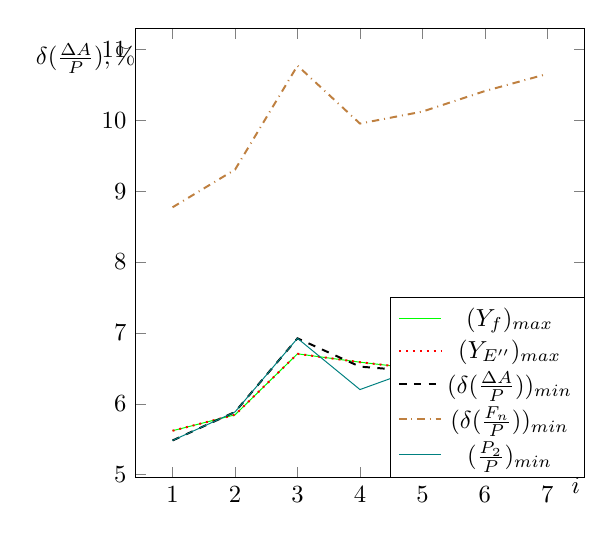
\begin{tikzpicture}[,
scale=0.89]
\begin{axis}[
  xlabel style = {{at={(axis description cs:.98,0.02)}}},
  ylabel = {$\delta(\frac{\Delta A}{P}), \%$},
  ylabel style = {{at={(axis description cs:-0.11,.88)},rotate=270,anchor=south}},
  xlabel = {$i$},
  width=8cm, height=8cm, xtick={1,2,3,4,5,6,7}, legend style={at={(1,0)},anchor=south east}
]

\addplot+[mark=none,
  solid, green, thin
] coordinates {
  (1.0, 5.619564224321039)
  (2.0, 5.84441657242741)
  (3.0, 6.704917867424845)
  (4.0, 6.586866390801599)
  (5.0, 6.485554729454776)
  (6.0, 6.754284481908828)
  (7.0, 6.998000929961407)
};
\addlegendentry{{}{$(Y_f)_\text{max}$}}

\addplot+[mark=none,
  dotted, red, thick
] coordinates {
  (1.0, 5.619564224321039)
  (2.0, 5.84441657242741)
  (3.0, 6.704917867424845)
  (4.0, 6.586866390801599)
  (5.0, 6.485554729454776)
  (6.0, 6.754284481908828)
  (7.0, 6.998000929961407)
};
\addlegendentry{{}{$(Y_{E''})_\text{max}$}}

\addplot+[mark=none,
  dashed, black, thick
] coordinates {
  (1.0, 5.482150178426482)
  (2.0, 5.884813687357447)
  (3.0, 6.923308229121754)
  (4.0, 6.524186589001574)
  (5.0, 6.4527000666451135)
  (6.0, 6.739088245807983)
  (7.0, 6.991066392896656)
};
\addlegendentry{{}{$(\delta(\frac{\Delta A}{P}))_\text{min}$}}

\addplot+[mark=none,
  dashdotted, brown, thick
] coordinates {
  (1.0, 8.771994897379303)
  (2.0, 9.303209789751323)
  (3.0, 10.770438360555245)
  (4.0, 9.953392791027085)
  (5.0, 10.122163189828624)
  (6.0, 10.411774829351534)
  (7.0, 10.654096806225095)
};
\addlegendentry{{}{$(\delta(\frac{F_n}{P}))_\text{min}$}}

\addplot+[mark=none,
  solid, teal, thin
] coordinates {
  (1.0, 5.482150178426482)
  (2.0, 5.884813687357447)
  (3.0, 6.923308229121754)
  (4.0, 6.2006153993959785)
  (5.0, 6.519171025702167)
  (6.0, 6.804418040883925)
  (7.0, 7.023084861927327)
};
\addlegendentry{{}{$(\frac{P_2}{P})_\text{min}$}}

\end{axis}
\end{tikzpicture}


%   \caption{{Зависимость экономии работы разделения в двойном каскаде с замыканием от номера перегрузки для различных критериев оптимальности. ($C_{235,{P}}=4,95\%$){\label{6}}}}
%   \end{minipage}
% \end{figure}
% \begin{figure}[ht]
%     \centering
%     \begin{minipage}{.51\textwidth}
%       \centering
%       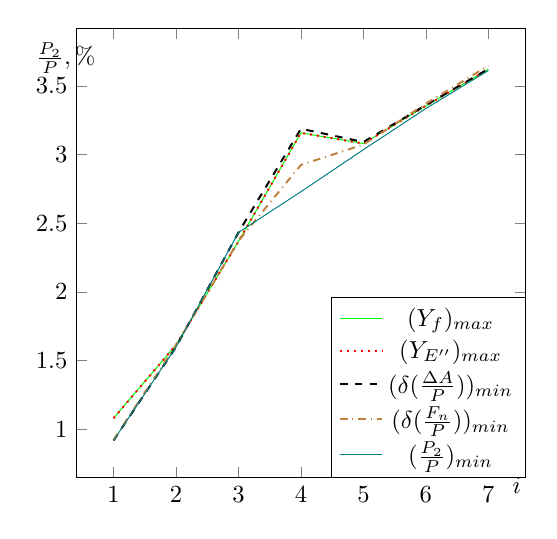
\begin{tikzpicture}[,
scale=0.89]
\begin{axis}[
  xlabel style = {{at={(axis description cs:.98,0.02)}}},
  ylabel = {$\frac{P_{2}}{P}, \%$},
  ylabel style = {{at={(axis description cs:-0.023,.88)},rotate=270,anchor=south}},
  xlabel = {$i$},
  width=8cm, height=8cm, xtick={1,2,3,4,5,6,7}, legend style={at={(1,0)},anchor=south east}
]

\addplot+[mark=none,
  solid, green, thin
] coordinates {
  (1.0, 1.0810960189992584)
  (2.0, 1.6146633333341598)
  (3.0, 2.3687024775347747)
  (4.0, 3.159113715125525)
  (5.0, 3.0809753572386254)
  (6.0, 3.3558969337102944)
  (7.0, 3.621806533418627)
};
\addlegendentry{{}{$(Y_f)_\text{max}$}}

\addplot+[mark=none,
  dotted, red, thick
] coordinates {
  (1.0, 1.0810960189992584)
  (2.0, 1.6146633333341598)
  (3.0, 2.3687024775347747)
  (4.0, 3.159113715125525)
  (5.0, 3.0809753572386254)
  (6.0, 3.3558969337102944)
  (7.0, 3.621806533418627)
};
\addlegendentry{{}{$(Y_{E''})_\text{max}$}}

\addplot+[mark=none,
  dashed, black, thick
] coordinates {
  (1.0, 0.9191318565385409)
  (2.0, 1.5995427357743446)
  (3.0, 2.4336632372639344)
  (4.0, 3.1886436788896333)
  (5.0, 3.0921075113377343)
  (6.0, 3.3608476613695917)
  (7.0, 3.6241033759848253)
};
\addlegendentry{{}{$(\delta(\frac{\Delta A}{P}))_\text{min}$}}

\addplot+[mark=none,
  dashdotted, brown, thick
] coordinates {
  (1.0, 0.9234810348382065)
  (2.0, 1.612721145807963)
  (3.0, 2.3724712118887568)
  (4.0, 2.9252605855990694)
  (5.0, 3.0737574380632946)
  (6.0, 3.3714004647467988)
  (7.0, 3.6482779696747203)
};
\addlegendentry{{}{$(\delta(\frac{F_n}{P}))_\text{min}$}}

\addplot+[mark=none,
  solid, teal, thin
] coordinates {
  (1.0, 0.9191318565385409)
  (2.0, 1.5995427357743446)
  (3.0, 2.4336632372639344)
  (4.0, 2.7304942598358695)
  (5.0, 3.036681544811821)
  (6.0, 3.3363360013335974)
  (7.0, 3.6127481585062196)
};
\addlegendentry{{}{$(\frac{P_2}{P})_\text{min}$}}

\end{axis}
\end{tikzpicture}


%       \caption{{Зависимость отношения потоков побочного ($P_2$) и финального продукта (товарного НОУ) от  номера перегрузки для различных критериев оптимальности. ($C_{235,{P}}=4,95\%$){\label{5}}}}
%     \end{minipage}%
%     \begin{minipage}{.5\textwidth}
%         \centering
%         \input{images/tex/loop1_Mk/loop_exR_0.0495}
%     \caption{{Зависимость степени извлечения $^{235}$U из исходного регенерата в двойном каскаде с замыканием от номера перегрузки для различных критериев оптимальности. ($C_{235,{P}}=4,95\%$){\label{4}}}}
%     \end{minipage}
% \end{figure}

% \begin{figure}[h]
%     \centering
%     \input{images/tex/loop1_Mk/loop_E_0.0495}
%     \caption{Зависимость отношения потоков исходного регенерата и финального продукта (товарного НОУ) от номера перегрузки для различных критериев эффективности. ($C_{235,{P}}=4,95\%$)}\label{7}
% \end{figure}

% \begin{figure}[h]
%     \centering
%     \begin{minipage}{.5\textwidth}
%       \centering
%       \input{images/tex/loop1_Mk/loop_E232_0.0495}
%       \caption{{Зависимость концентрации $^{232}$U в исходном регенерате от номера перегрузки для различных критериев эффективности. ($C_{235,{P}}=4,95\%$){\label{8}}}}
%     \end{minipage}%
%     \begin{minipage}{.5\textwidth}
%       \centering
%       \input{images/tex/loop1_Mk/loop_E234_0.0495}
% \caption{{Зависимость концентрации $^{234}$U в исходном регенерате от номера перегрузки для различных критериев эффективности. ($C_{235,{P}}=4,95\%$){\label{9}}}}
% \end{minipage}
% \end{figure}

% \begin{figure}[h]
%     \centering
%     \begin{minipage}{.5\textwidth}
%       \centering
%       \input{images/tex/loop1_Mk/loop_E235_0.0495}
%       \caption{{Зависимость концентрации $^{235}$U в исходном регенерате от номера перегрузки для различных критериев эффективности. ($C_{235,{P}}=4,95\%$){\label{10}}}}
%     \end{minipage}%
%     \begin{minipage}{.5\textwidth}
%       \centering
%       \input{images/tex/loop1_Mk/loop_E236_0.0495}
% \caption{{Зависимость концентрации $^{236}$U в исходном регенерате от номера перегрузки для различных критериев эффективности. ($C_{235,{P}}=4,95\%$){\label{11}}}}
% \end{minipage}
% \end{figure}

















































% Для демонстрации возможностей, получаемых применением предложенных в диссертации методик оптимизации, представим серию расчетов тройного каскада с НОУ-разбавителем, получив интегральные показатели для различных оптимизационных критериев.

% \begin{table}
%     \begin{tabular}{ccccc}
%         $\cdot$ & $(Y_f)_\text{max}$ & $(Y_{E})_\text{max}$ & $(\delta(\frac{\Delta A}{P}))_\text{min}$ & $(\delta(\frac{F_n}{P}))_\text{min}$\\ \hline
%         $\text{Сумм. степень изв-я}$ & $0.778$ & $0.07535$ & $0.07535$ & $0.03058$\\ \hline
%         $\text{Степень изв-я из рег-та}$ & $0.7976$ & $0.8765$ & $0.8765$ & $0.7504$\\ \hline
%         $\text{Потери РР, \%}$ & $6.814$ & $-1.127$ & $-1.127$ & $137.4$\\ \hline
%         $\text{Расх. пр. U на ед. прод.}$ & $6.217$ & $6.246$ & $6.246$ & $0.922$\\ \hline
%         $\text{Эк. пр. U, \%}$ & $21.62$ & $21.24$ & $21.24$ & $88.38$\\ \hline
%         $C_{235,P_1, \%}$ & $5.0$ & $5.0$ & $5.0$ & $15.0$\\ \hline
%         $C_{235,W_2, \%}$ & $4.227$ & $4.708$ & $4.708$ & $14.1$\\ \hline
%         $C_{235,P_0, \%}$ & $5.425$ & $5.321$ & $5.321$ & $5.456$\\ \hline
%         $C_{235,P_2, \%}$ & $16.0$ & $20.0$ & $20.0$ & $20.0$\\ \hline
%         $C_{232,P_1, \%}$ & $2.443e-6$ & $2.443e-6$ & $2.443e-6$ & $7.431e-6$\\ \hline
%         $C_{232,W_2, \%}$ & $1.515e-6$ & $1.998e-6$ & $1.998e-6$ & $6.329e-6$\\ \hline
%         $C_{232,P_2, \%}$ & $1.564e-5$ & $2.526e-5$ & $2.526e-5$ & $1.357e-5$\\ \hline
%         $C_{234,P_1, \%}$ & $0.1198$ & $0.1198$ & $0.1198$ & $0.3672$\\ \hline
%         $C_{234,W_2, \%}$ & $0.09223$ & $0.1084$ & $0.1084$ & $0.3349$\\ \hline
%         $C_{234,P_2, \%}$ & $0.512$ & $0.7049$ & $0.7049$ & $0.5472$\\ \hline
%         $C_{236,P_1, \%}$ & $2.942$ & $2.942$ & $2.942$ & $6.159$\\ \hline
%         $C_{236,W_2, \%}$ & $2.69$ & $2.856$ & $2.856$ & $5.955$\\ \hline
%         $\text{Уд. сумм. поток к-а 2}$ & $6.009$ & $2.627$ & $2.627$ & $0.2777$\\ \hline
%         $\text{Уд. сумм. поток доп. к-а}$ & $2285.0$ & $2285.0$ & $2285.0$ & $339.3$\\ \hline
%         $\text{Доля P2 в F3}$ & $0.002519$ & $1.0e-5$ & $1.0e-5$ & $1.0e-5$\\ \hline
%         $\text{U-235 в W3, \%}$ & $0.13$ & $0.13$ & $0.13$ & $0.1275$\\ \hline
%         $\text{U-235 в P3, \%}$ & $5.319$ & $4.617$ & $4.617$ & $4.253$\\ \hline
%         $\text{Р3, кг}$ & $74.86$ & $31.42$ & $31.42$ & $1219.0$\\ \hline
%         $\text{U-232, \%}$ & $5.0e-7$ & $4.945e-7$ & $4.945e-7$ & $4.552e-7$\\ \hline
%         $\text{U-234, \%}$ & $0.05795$ & $0.05973$ & $0.05973$ & $0.04356$\\ \hline
%         $\text{U-235, \%}$ & $5.137$ & $5.155$ & $5.155$ & $5.072$\\ \hline
%         $\text{U-236, \%}$ & $0.6463$ & $0.706$ & $0.706$ & $0.4194$\\ \hline
%         $F_{P_1}, \text{кг}$ & $372.8$ & $372.8$ & $372.8$ & $122.6$\\ \hline
%         $F_{W_2}, \text{кг}$ & $348.3$ & $365.6$ & $365.6$ & $103.9$\\ \hline
%         $F_{P_0}, \text{кг}$ & $1056.0$ & $1082.0$ & $1082.0$ & $155.7$\\ \hline
%         $F_{P_2}, \text{кг}$ & $24.48$ & $7.127$ & $7.127$ & $18.64$\\ \hline
%         \end{tabular}        
% \caption{Параметры схемы тройного каскада с НОУ-разбавителем при различных критериях оптимизации для обогащения регенерата второго рецикла.{\label{3opt2}}}
% \end{table}

% Анализируя результаты, представленные в \ref{3opt2}, заметим, что для оптимумов извлечения  $^{235}$U из регенерата и расхода работы разделения полученые решения идентичны. Эти решения позволяют вовлечь регенерат второго рецикла в ЯТЦ, оптимальным образом извлекая  $^{235}$U, выигрывая по этому показателю двойную схему, где $P_2$ не используется в производстве НОУ-продукта, не затрачивая дополнительную работу разделения по сравнению со схемой ординарного каскада для обогащения природного урана.
% Схема также позволяет найти решения, минимизирующие расход природного урана, в которых его затраты на единицу продукта будут на порядок меньше, однако это достигается за счет высокого расхода ОГФУ, и как следствие, больших потерь работы разделения (>100\%), а также ухудшения извлечения  $^{235}$U. 

% \begin{table}
%     \begin{tabular}{ccccc}
%         $\cdot$ & $(Y_f)_\text{max}$ & $(Y_{E})_\text{max}$ & $(\delta(\frac{\Delta A}{P}))_\text{min}$ & $(\delta(\frac{F_n}{P}))_\text{min}$\\ \hline
%         $\text{Сумм. степень изв-я}$ & $0.7531$ & $0.04262$ & $0.7531$ & $0.02461$\\ \hline
%         $\text{Степень изв-я из рег-та}$ & $0.05408$ & $0.7628$ & $0.05408$ & $0.648$\\ \hline
%         $\text{Потери РР, \%}$ & $-0.4811$ & $11.38$ & $-0.4811$ & $173.3$\\ \hline
%         $\text{Расх. пр. U на ед. прод.}$ & $7.866$ & $6.882$ & $7.866$ & $0.2052$\\ \hline
%         $\text{Эк. пр. U, \%}$ & $0.8189$ & $13.23$ & $0.8189$ & $97.41$\\ \hline
%         $C_{235,P_1, \%}$ & $5.095$ & $5.0$ & $5.095$ & $9.0$\\ \hline
%         $C_{235,W_2, \%}$ & $4.923$ & $4.334$ & $4.923$ & $7.583$\\ \hline
%         $C_{235,P_0, \%}$ & $4.963$ & $5.428$ & $4.963$ & $4.736$\\ \hline
%         $C_{235,P_2, \%}$ & $16.0$ & $18.0$ & $16.0$ & $16.0$\\ \hline
%         $C_{232,P_1, \%}$ & $1.425e-5$ & $5.191e-6$ & $1.425e-5$ & $9.429e-6$\\ \hline
%         $C_{232,W_2, \%}$ & $1.257e-5$ & $2.852e-6$ & $1.257e-5$ & $5.601e-6$\\ \hline
%         $C_{232,P_2, \%}$ & $0.0001205$ & $5.087e-5$ & $0.0001205$ & $2.834e-5$\\ \hline
%         $C_{234,P_1, \%}$ & $0.2841$ & $0.1944$ & $0.2841$ & $0.3528$\\ \hline
%         $C_{234,W_2, \%}$ & $0.2681$ & $0.1507$ & $0.2681$ & $0.2694$\\ \hline
%         $C_{234,P_2, \%}$ & $1.295$ & $1.048$ & $1.295$ & $0.765$\\ \hline
%         $C_{236,P_1, \%}$ & $4.239$ & $5.446$ & $4.239$ & $9.226$\\ \hline
%         $C_{236,W_2, \%}$ & $4.167$ & $5.095$ & $4.167$ & $8.432$\\ \hline
%         $C_{236,P_2, \%}$ & $8.804$ & $12.3$ & $8.804$ & $13.14$\\ \hline
%         $M_{k1}$ & $234$ & $238$ & $234$ & $238$\\ \hline
%         $M_{k2}$ & $232$ & $232$ & $232$ & $232$\\ \hline
%         $\text{Уд. сумм. поток к-а 1}$ & $7.501$ & $371.5$ & $7.501$ & $441.2$\\ \hline
%         $\text{Уд. сумм. поток к-а 2}$ & $0.06838$ & $6.21$ & $0.06838$ & $1.869$\\ \hline
%         $\text{Уд. сумм. поток доп. к-а}$ & $2828.0$ & $2530.0$ & $2828.0$ & $72.87$\\ \hline
%         $\text{Доля P2 в F3}$ & $0.25$ & $1.0e-5$ & $0.25$ & $1.062e-5$\\ \hline
%         $\text{U-235 в W3, \%}$ & $0.105$ & $0.13$ & $0.105$ & $0.1275$\\ \hline
%         $\text{U-235 в P3, \%}$ & $4.896$ & $4.616$ & $4.896$ & $4.939$\\ \hline
%         $\text{Р3, кг}$ & $0.8097$ & $52.46$ & $0.8097$ & $1315.0$\\ \hline
%         $\text{U-232, \%}$ & $1.502e-7$ & $5.0e-7$ & $1.502e-7$ & $5.0e-7$\\ \hline
%         $\text{U-234, \%}$ & $0.04393$ & $0.06286$ & $0.04393$ & $0.04301$\\ \hline
%         $\text{U-235, \%}$ & $4.963$ & $5.208$ & $4.963$ & $5.156$\\ \hline
%         $\text{U-236, \%}$ & $0.04464$ & $0.89$ & $0.04464$ & $0.7112$\\ \hline
%         $F_{P_1}, \text{кг}$ & $15.59$ & $271.6$ & $15.59$ & $149.5$\\ \hline
%         $F_{W_2}, \text{кг}$ & $15.35$ & $258.4$ & $15.35$ & $124.4$\\ \hline
%         $F_{P_0}, \text{кг}$ & $1463.0$ & $1168.0$ & $1463.0$ & $40.04$\\ \hline
%         $F_{P_2}, \text{кг}$ & $0.2429$ & $13.23$ & $0.2429$ & $25.17$\\ \hline
%         \end{tabular}
% \caption{Параметры схемы тройного каскада с НОУ-разбавителем при различных критериях оптимизации для обогащения регенерата пятого рецикла.{\label{3opt5}}}
% \end{table}


% Анализируя результаты, представленные в \ref{3opt5}, заметим, что для оптимумов суммарной степени извлечения $^{235}$U из регенерата и расхода работы разделения полученые решения идентичны. Однако для них наблюдается низкая степень извлечения $^{235}$U из регенерата $\approx$5\%. При этом в решении с оптимумом извлечения $^{235}$U из регенерата, очень низка интегральная степень извлечения $^{235}$U  и составляет $\approx$5\%. 


% \begin{table}[h]
% \centering
% \begin{tabular}{ccc}
%     $\text{Каскад | П-р}$ & $\text{Уд. расход р-та}$ & $\text{ЕРР}$\\ \hline
%     $\text{С доп. питанием}$ & $0.01686$ & $11.82$\\ \hline
%     $\text{С доп. продуктом}$ & $0.07994$ & $11.95$\\ \hline
%     $\text{С доп. потоком питания}$ & $0.7552$ & $10.81$
% \end{tabular}\caption{{Параметры каскадов.{\label{table_ords}}}}
% \end{table}

% \begin{table}[h]
%     \centering
%     \begin{tabular}{|c|c|c|c|c|c|}
%     $\text{Каскад}$ & $\text{Экономия ЕРР,\%}$ & $\text{Уд.расход Регенерата,\%}$ & $\text{Уд.расход ОГФУ,\%}$ & $\text{Теор.стоимость,\%}$\\ \hline
%     1&7.31&1.04&0.49&0&92.71\\
%     2&100&41.63&8.26&0&0.32\\
%     3&10.07&6.08&0.93&0&89.96\\
%     4&15.08&25&0.93&31.11&85.00\\
%     4&23.13&50&0.93&74.49&77.02\\
%     \end{tabular}\caption{\label{from_splg19}Таблица сравнения каскадов.}
% \end{table}

% \textbf{Схема двойного каскада с НОУ-разбавителем с возвратом потока $P_2$ в цикл. Дополнительные результаты для состава 1}


% На рисунок \ref{3}-\ref{4} представлены зависимости, отражающие зависимость ключевых показателей эффективности схемы при различных оптимизационных критериях: $(Y_f)_\text{max}$, $(Y_{E''})_\text{max}$, $(\delta(\frac{\Delta A}{P}))_\text{min}$, $(\delta(\frac{F_n}{P}))_\text{min}$, $(\frac{P_2}{P})_\text{min}$ от номера перегрузки.

% \begin{figure}[ht]
%     \centering
%     \begin{minipage}{.5\textwidth}
%       \centering
%       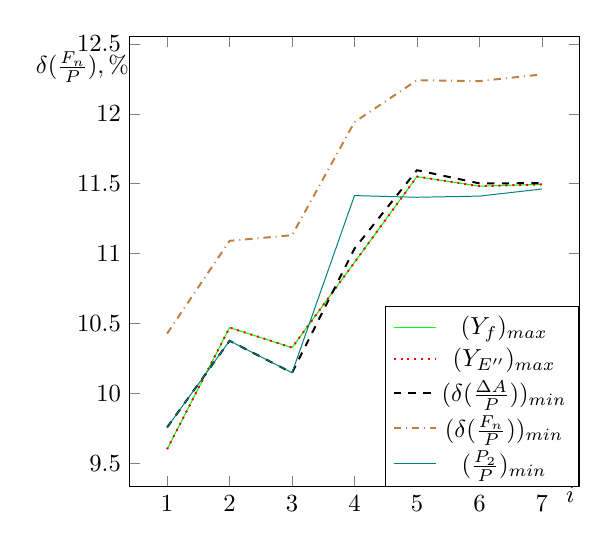
\begin{tikzpicture}[,
scale=0.89]
\begin{axis}[
  xlabel style = {{at={(axis description cs:.98,0.02)}}},
  ylabel = {$\delta(\frac{F_n}{P}), \%$},
  ylabel style = {{at={(axis description cs:-0.105,.88)},rotate=270,anchor=south}},
  xlabel = {$i$},
  width=8cm, height=8cm, xtick={1,2,3,4,5,6,7}, legend style={at={(1,0)},anchor=south east}
]

\addplot+[mark=none,
  solid, green, thin
] coordinates {
  (1.0, 9.60224940765123)
  (2.0, 10.471964607421514)
  (3.0, 10.328677265019726)
  (4.0, 10.937722799772365)
  (5.0, 11.551073258460454)
  (6.0, 11.482634526238378)
  (7.0, 11.495414262020132)
};
\addlegendentry{{}{$(Y_f)_\text{max}$}}

\addplot+[mark=none,
  dotted, red, thick
] coordinates {
  (1.0, 9.60224940765123)
  (2.0, 10.471964607421514)
  (3.0, 10.328677265019726)
  (4.0, 10.937722799772365)
  (5.0, 11.551073258460454)
  (6.0, 11.482634526238378)
  (7.0, 11.495414262020132)
};
\addlegendentry{{}{$(Y_{E''})_\text{max}$}}

\addplot+[mark=none,
  dashed, black, thick
] coordinates {
  (1.0, 9.758344663807906)
  (2.0, 10.377586059230682)
  (3.0, 10.148945832377942)
  (4.0, 11.036603656094378)
  (5.0, 11.596700175896046)
  (6.0, 11.502422364899322)
  (7.0, 11.5042389394856)
};
\addlegendentry{{}{$(\delta(\frac{\Delta A}{P}))_\text{min}$}}

\addplot+[mark=none,
  dashdotted, brown, thick
] coordinates {
  (1.0, 10.428757919569875)
  (2.0, 11.091940883100326)
  (3.0, 11.132231272182302)
  (4.0, 11.940825541138867)
  (5.0, 12.240045586112991)
  (6.0, 12.233596137265634)
  (7.0, 12.281186997924387)
};
\addlegendentry{{}{$(\delta(\frac{F_n}{P}))_\text{min}$}}

\addplot+[mark=none,
  solid, teal, thin
] coordinates {
  (1.0, 9.758344663807906)
  (2.0, 10.377586059230682)
  (3.0, 10.148945832377942)
  (4.0, 11.415331124937522)
  (5.0, 11.403205816515582)
  (6.0, 11.411528711119201)
  (7.0, 11.462271406331004)
};
\addlegendentry{{}{$(\frac{P_2}{P})_\text{min}$}}

\end{axis}
\end{tikzpicture}


%       \caption{{Зависимость экономии природного урана в двойном каскаде с замыканием от номера перегрузки для различных критериев оптимальности. ($C_{235,{P}}=4,95\%$){\label{3}}}}
%     \end{minipage}%
%     \begin{minipage}{.5\textwidth}
%         \centering
%         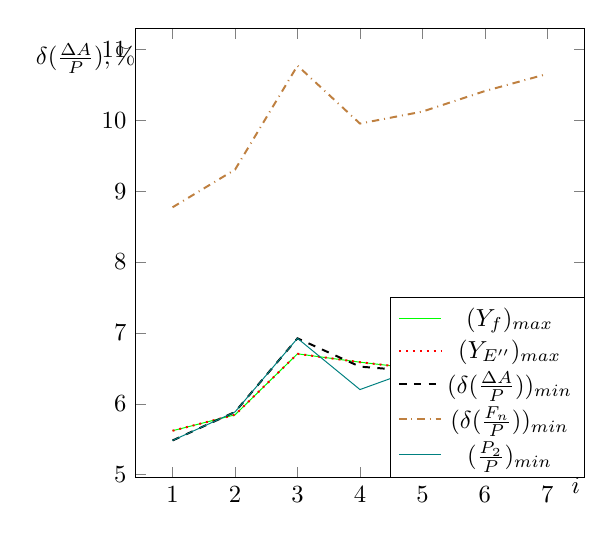
\begin{tikzpicture}[,
scale=0.89]
\begin{axis}[
  xlabel style = {{at={(axis description cs:.98,0.02)}}},
  ylabel = {$\delta(\frac{\Delta A}{P}), \%$},
  ylabel style = {{at={(axis description cs:-0.11,.88)},rotate=270,anchor=south}},
  xlabel = {$i$},
  width=8cm, height=8cm, xtick={1,2,3,4,5,6,7}, legend style={at={(1,0)},anchor=south east}
]

\addplot+[mark=none,
  solid, green, thin
] coordinates {
  (1.0, 5.619564224321039)
  (2.0, 5.84441657242741)
  (3.0, 6.704917867424845)
  (4.0, 6.586866390801599)
  (5.0, 6.485554729454776)
  (6.0, 6.754284481908828)
  (7.0, 6.998000929961407)
};
\addlegendentry{{}{$(Y_f)_\text{max}$}}

\addplot+[mark=none,
  dotted, red, thick
] coordinates {
  (1.0, 5.619564224321039)
  (2.0, 5.84441657242741)
  (3.0, 6.704917867424845)
  (4.0, 6.586866390801599)
  (5.0, 6.485554729454776)
  (6.0, 6.754284481908828)
  (7.0, 6.998000929961407)
};
\addlegendentry{{}{$(Y_{E''})_\text{max}$}}

\addplot+[mark=none,
  dashed, black, thick
] coordinates {
  (1.0, 5.482150178426482)
  (2.0, 5.884813687357447)
  (3.0, 6.923308229121754)
  (4.0, 6.524186589001574)
  (5.0, 6.4527000666451135)
  (6.0, 6.739088245807983)
  (7.0, 6.991066392896656)
};
\addlegendentry{{}{$(\delta(\frac{\Delta A}{P}))_\text{min}$}}

\addplot+[mark=none,
  dashdotted, brown, thick
] coordinates {
  (1.0, 8.771994897379303)
  (2.0, 9.303209789751323)
  (3.0, 10.770438360555245)
  (4.0, 9.953392791027085)
  (5.0, 10.122163189828624)
  (6.0, 10.411774829351534)
  (7.0, 10.654096806225095)
};
\addlegendentry{{}{$(\delta(\frac{F_n}{P}))_\text{min}$}}

\addplot+[mark=none,
  solid, teal, thin
] coordinates {
  (1.0, 5.482150178426482)
  (2.0, 5.884813687357447)
  (3.0, 6.923308229121754)
  (4.0, 6.2006153993959785)
  (5.0, 6.519171025702167)
  (6.0, 6.804418040883925)
  (7.0, 7.023084861927327)
};
\addlegendentry{{}{$(\frac{P_2}{P})_\text{min}$}}

\end{axis}
\end{tikzpicture}


%   \caption{{Зависимость экономии работы разделения в двойном каскаде с замыканием от номера перегрузки для различных критериев оптимальности. ($C_{235,{P}}=4,95\%$){\label{6}}}}
%   \end{minipage}
% \end{figure}

% \begin{figure}[ht]
%     \centering
%     \begin{minipage}{.51\textwidth}
%       \centering
%       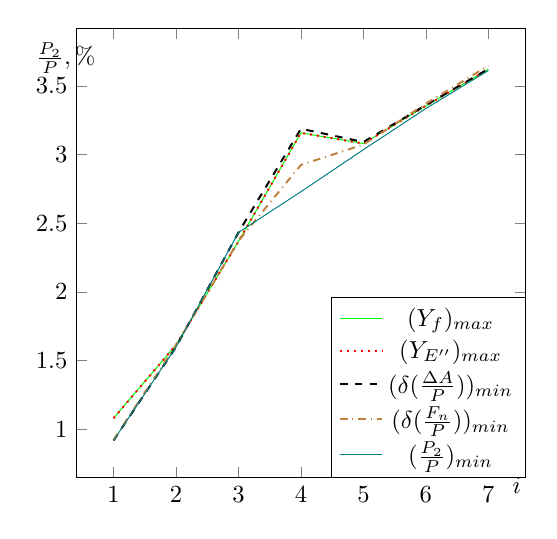
\begin{tikzpicture}[,
scale=0.89]
\begin{axis}[
  xlabel style = {{at={(axis description cs:.98,0.02)}}},
  ylabel = {$\frac{P_{2}}{P}, \%$},
  ylabel style = {{at={(axis description cs:-0.023,.88)},rotate=270,anchor=south}},
  xlabel = {$i$},
  width=8cm, height=8cm, xtick={1,2,3,4,5,6,7}, legend style={at={(1,0)},anchor=south east}
]

\addplot+[mark=none,
  solid, green, thin
] coordinates {
  (1.0, 1.0810960189992584)
  (2.0, 1.6146633333341598)
  (3.0, 2.3687024775347747)
  (4.0, 3.159113715125525)
  (5.0, 3.0809753572386254)
  (6.0, 3.3558969337102944)
  (7.0, 3.621806533418627)
};
\addlegendentry{{}{$(Y_f)_\text{max}$}}

\addplot+[mark=none,
  dotted, red, thick
] coordinates {
  (1.0, 1.0810960189992584)
  (2.0, 1.6146633333341598)
  (3.0, 2.3687024775347747)
  (4.0, 3.159113715125525)
  (5.0, 3.0809753572386254)
  (6.0, 3.3558969337102944)
  (7.0, 3.621806533418627)
};
\addlegendentry{{}{$(Y_{E''})_\text{max}$}}

\addplot+[mark=none,
  dashed, black, thick
] coordinates {
  (1.0, 0.9191318565385409)
  (2.0, 1.5995427357743446)
  (3.0, 2.4336632372639344)
  (4.0, 3.1886436788896333)
  (5.0, 3.0921075113377343)
  (6.0, 3.3608476613695917)
  (7.0, 3.6241033759848253)
};
\addlegendentry{{}{$(\delta(\frac{\Delta A}{P}))_\text{min}$}}

\addplot+[mark=none,
  dashdotted, brown, thick
] coordinates {
  (1.0, 0.9234810348382065)
  (2.0, 1.612721145807963)
  (3.0, 2.3724712118887568)
  (4.0, 2.9252605855990694)
  (5.0, 3.0737574380632946)
  (6.0, 3.3714004647467988)
  (7.0, 3.6482779696747203)
};
\addlegendentry{{}{$(\delta(\frac{F_n}{P}))_\text{min}$}}

\addplot+[mark=none,
  solid, teal, thin
] coordinates {
  (1.0, 0.9191318565385409)
  (2.0, 1.5995427357743446)
  (3.0, 2.4336632372639344)
  (4.0, 2.7304942598358695)
  (5.0, 3.036681544811821)
  (6.0, 3.3363360013335974)
  (7.0, 3.6127481585062196)
};
\addlegendentry{{}{$(\frac{P_2}{P})_\text{min}$}}

\end{axis}
\end{tikzpicture}


%       \caption{{Зависимость отношения потоков побочного ($P_2$) и финального продукта (товарного НОУ) от  номера перегрузки для различных критериев оптимальности. ($C_{235,{P}}=4,95\%$){\label{5}}}}
%     \end{minipage}%
%     \begin{minipage}{.5\textwidth}
%         \centering
%         \input{images/tex/loop1/loop_exR_0.0495}
%     \caption{{Зависимость степени извлечения $^{235}$U из исходного регенерата в двойном каскаде с замыканием от номера перегрузки для различных критериев оптимальности. ($C_{235,{P}}=4,95\%$){\label{4}}}}
%     \end{minipage}
% \end{figure}

% Как можно заметить, общей тенденцией для всех случаев является снижение эффективности схемы по каждому из показателей. Например, можно видеть, что происходит уменьшение степени извлечения $^{235}$U из регенерата на каждой последующей перегрузке, что обуславливает также и увеличение перерасхода работы разделения. Эти эффекты являются следствием повышения с каждой перегрузкой концентрации четных изотопов в питающем первый каскад регенерате и массы самого регенерата. Эти утверждения иллюстрируют рисунок \ref{7}-\ref{10}, отражающие изменений величины $E/P$ и концентраций изотопов $^{235}$U и $^{232,234,236}$U в потоке обогащаемого регенерата после его смешивания с отходом обогащения регенерата для предыдущей перегрузки. Как видно, из указанных рисунков, концентрации четных изотопов, особенно $^{232,234}$U, существенно (в несколько раз) возрастают от первой перегрузки к седьмой. Так, концентрация $^{232}$U достигает значений $\approx 4\cdot10^{-6} \%$, что в восемь раз больше, чем предельное значение для товарного НОУ. При этом на 0,5--0,6 \% возрастает концентрация $^{235}$U, что и обеспечивает снижение расхода природного урана.       

% \begin{figure}[h]
%     \centering
%     \input{images/tex/loop1/loop_E_0.0495}
%     \caption{Зависимость отношения потоков исходного регенерата и финального продукта (товарного НОУ) от номера перегрузки для различных критериев эффективности. ($C_{235,{P}}=4,95\%$)}\label{7}
% \end{figure}

% % \begin{figure}[h]
% %     \centering
% %     \input{images/tex/loop1/loop_sw_epp_0.0495}
% %     \caption{Зависимость отношения потоков исходного регенерата и финального продукта (товарного НОУ) от номера перегрузки для различных критериев эффективности. ($C_{235,{P}}=4,95\%$)}\label{777}
% % \end{figure}

% \begin{figure}[h]
%     \centering
%     \begin{minipage}{.5\textwidth}
%       \centering
%       \input{images/tex/loop1/loop_E232_0.0495}
%       \caption{{Зависимость концентрации $^{232}$U в исходном регенерате от номера перегрузки для различных критериев эффективности. ($C_{235,{P}}=4,95\%$){\label{8}}}}
%     \end{minipage}%
%     \begin{minipage}{.5\textwidth}
%       \centering
%       \input{images/tex/loop1/loop_E234_0.0495}
% \caption{{Зависимость концентрации $^{234}$U в исходном регенерате от номера перегрузки для различных критериев эффективности. ($C_{235,{P}}=4,95\%$){\label{9}}}}
% \end{minipage}
% \end{figure}

% \begin{figure}[h]
%     \centering
%     \begin{minipage}{.5\textwidth}
%       \centering
%       \input{images/tex/loop1/loop_E235_0.0495}
%       \caption{{Зависимость концентрации $^{235}$U в исходном регенерате от номера перегрузки для различных критериев эффективности. ($C_{235,{P}}=4,95\%$){\label{10}}}}
%     \end{minipage}%
%     \begin{minipage}{.5\textwidth}
%       \centering
%       \input{images/tex/loop1/loop_E236_0.0495}
% \caption{{Зависимость концентрации $^{236}$U в исходном регенерате от номера перегрузки для различных критериев эффективности. ($C_{235,{P}}=4,95\%$){\label{11}}}}
% \end{minipage}
% \end{figure}